\ifdefined\included
\else
\documentclass[a4paper,11pt,twoside]{StyleThese}
\usepackage{amsmath,amssymb}             % AMS Math
\usepackage[french]{babel}
\usepackage[utf8]{inputenc}
\usepackage[T1]{fontenc}
\usepackage{tabularx}
%\usepackage{tabular}
\usepackage{multirow}


\usepackage[tight,footnotesize]{subfigure}
\usepackage{algorithm} %To allow algorithm environment
\usepackage{algpseudocode} %Provides algorithmic environment

\usepackage{hhline}
\usepackage[left=1.5in,right=1.3in,top=1.1in,bottom=1.1in,includefoot,includehead,headheight=13.6pt]{geometry}
\renewcommand{\baselinestretch}{1.05}

% Table of contents for each chapter

\usepackage[nottoc, notlof, notlot]{tocbibind}
\usepackage[french]{minitoc}
\setcounter{minitocdepth}{2}
\mtcindent=15pt
% Use \minitoc where to put a table of contents

\usepackage{aecompl}

% Glossary / list of abbreviations

\usepackage[intoc]{nomencl}
\renewcommand{\nomname}{Liste des Abréviations}

\makenomenclature

% My pdf code

\usepackage{ifpdf}

\ifpdf
  \usepackage[pdftex]{graphicx}
  \DeclareGraphicsExtensions{.jpg}
  \usepackage[a4paper,pagebackref,hyperindex=true]{hyperref}
  \usepackage{tikz}
  \usetikzlibrary{arrows,shapes,calc}
\else
  \usepackage{graphicx}
  \DeclareGraphicsExtensions{.ps,.eps}
  \usepackage[a4paper,dvipdfm,pagebackref,hyperindex=true]{hyperref}
\fi

\graphicspath{{.}{images/}}

%nicer backref links
\renewcommand*{\backref}[1]{}
\renewcommand*{\backrefalt}[4]{%
\ifcase #1 %
(Non cité.)%
\or
(Cité en page~#2.)%
\else
(Cité en pages~#2.)%
\fi}
\renewcommand*{\backrefsep}{, }
\renewcommand*{\backreftwosep}{ et~}
\renewcommand*{\backreflastsep}{ et~}

% Links in pdf
\usepackage{color}
\definecolor{linkcol}{rgb}{0,0,0.4} 
\definecolor{citecol}{rgb}{0.5,0,0} 
\definecolor{linkcol}{rgb}{0,0,0} 
\definecolor{citecol}{rgb}{0,0,0}
% Change this to change the informations included in the pdf file

\hypersetup
{
bookmarksopen=true,
pdftitle="Évaluation de la sécurité des équipements grand public connectés à Internet",
pdfauthor="Yann BACHY", %auteur du document
pdfsubject="Thèse", %sujet du document
%pdftoolbar=false, %barre d'outils non visible
pdfmenubar=true, %barre de menu visible
pdfhighlight=/O, %effet d'un clic sur un lien hypertexte
colorlinks=true, %couleurs sur les liens hypertextes
pdfpagemode=None, %aucun mode de page
pdfpagelayout=SinglePage, %ouverture en simple page
pdffitwindow=true, %pages ouvertes entierement dans toute la fenetre
linkcolor=linkcol, %couleur des liens hypertextes internes
citecolor=citecol, %couleur des liens pour les citations
urlcolor=linkcol %couleur des liens pour les url
}

% definitions.
% -------------------

\setcounter{secnumdepth}{3}
\setcounter{tocdepth}{2}

% Some useful commands and shortcut for maths:  partial derivative and stuff

\newcommand{\pd}[2]{\frac{\partial #1}{\partial #2}}
\def\abs{\operatorname{abs}}
\def\argmax{\operatornamewithlimits{arg\,max}}
\def\argmin{\operatornamewithlimits{arg\,min}}
\def\diag{\operatorname{Diag}}
\newcommand{\eqRef}[1]{(\ref{#1})}

\usepackage{rotating}                    % Sideways of figures & tables
%\usepackage{bibunits}
%\usepackage[sectionbib]{chapterbib}          % Cross-reference package (Natural BiB)
%\usepackage{natbib}                  % Put References at the end of each chapter
                                         % Do not put 'sectionbib' option here.
                                         % Sectionbib option in 'natbib' will do.
\usepackage{fancyhdr}                    % Fancy Header and Footer

% \usepackage{txfonts}                     % Public Times New Roman text & math font
  
%%% Fancy Header %%%%%%%%%%%%%%%%%%%%%%%%%%%%%%%%%%%%%%%%%%%%%%%%%%%%%%%%%%%%%%%%%%
% Fancy Header Style Options

\pagestyle{fancy}                       % Sets fancy header and footer
\fancyfoot{}                            % Delete current footer settings

%\renewcommand{\chaptermark}[1]{         % Lower Case Chapter marker style
%  \markboth{\chaptername\ \thechapter.\ #1}}{}} %

%\renewcommand{\sectionmark}[1]{         % Lower case Section marker style
%  \markright{\thesection.\ #1}}         %

\fancyhead[LE,RO]{\bfseries\thepage}    % Page number (boldface) in left on even
% pages and right on odd pages
\fancyhead[RE]{\bfseries\nouppercase{\leftmark}}      % Chapter in the right on even pages
\fancyhead[LO]{\bfseries\nouppercase{\rightmark}}     % Section in the left on odd pages

\let\headruleORIG\headrule
\renewcommand{\headrule}{\color{black} \headruleORIG}
\renewcommand{\headrulewidth}{1.0pt}
\usepackage{colortbl}
\arrayrulecolor{black}

\fancypagestyle{plain}{
  \fancyhead{}
  \fancyfoot{}
  \renewcommand{\headrulewidth}{0pt}
}

%\usepackage{MyAlgorithm}
%\usepackage[noend]{MyAlgorithmic}
\usepackage[ED=MITT - STICIA, Ets=INP]{tlsflyleaf}
%%% Clear Header %%%%%%%%%%%%%%%%%%%%%%%%%%%%%%%%%%%%%%%%%%%%%%%%%%%%%%%%%%%%%%%%%%
% Clear Header Style on the Last Empty Odd pages
\makeatletter

\def\cleardoublepage{\clearpage\if@twoside \ifodd\c@page\else%
  \hbox{}%
  \thispagestyle{empty}%              % Empty header styles
  \newpage%
  \if@twocolumn\hbox{}\newpage\fi\fi\fi}

\makeatother
 
%%%%%%%%%%%%%%%%%%%%%%%%%%%%%%%%%%%%%%%%%%%%%%%%%%%%%%%%%%%%%%%%%%%%%%%%%%%%%%% 
% Prints your review date and 'Draft Version' (From Josullvn, CS, CMU)
\newcommand{\reviewtimetoday}[2]{\special{!userdict begin
    /bop-hook{gsave 20 710 translate 45 rotate 0.8 setgray
      /Times-Roman findfont 12 scalefont setfont 0 0   moveto (#1) show
      0 -12 moveto (#2) show grestore}def end}}
% You can turn on or off this option.
% \reviewtimetoday{\today}{Draft Version}
%%%%%%%%%%%%%%%%%%%%%%%%%%%%%%%%%%%%%%%%%%%%%%%%%%%%%%%%%%%%%%%%%%%%%%%%%%%%%%% 

\newenvironment{maxime}[1]
{
\vspace*{0cm}
\hfill
\begin{minipage}{0.5\textwidth}%
%\rule[0.5ex]{\textwidth}{0.1mm}\\%
\hrulefill $\:$ {\bf #1}\\
%\vspace*{-0.25cm}
\it 
}%
{%

\hrulefill
\vspace*{0.5cm}%
\end{minipage}
}

\let\minitocORIG\minitoc
\renewcommand{\minitoc}{\minitocORIG \vspace{1.5em}}

\usepackage{multirow}
%\usepackage{slashbox}

\newenvironment{bulletList}%
{ \begin{list}%
	{$\bullet$}%
	{\setlength{\labelwidth}{25pt}%
	 \setlength{\leftmargin}{30pt}%
	 \setlength{\itemsep}{\parsep}}}%
{ \end{list} }

\newtheorem{definition}{Définition}
\renewcommand{\epsilon}{\varepsilon}

% centered page environment

\newenvironment{vcenterpage}
{\newpage\vspace*{\fill}\thispagestyle{empty}\renewcommand{\headrulewidth}{0pt}}
{\vspace*{\fill}}

\usepackage{tablefootnote}
\sloppy


\begin{document}
\setcounter{chapter}{4} %% Numéro du chapitre précédent ;)
\dominitoc
\faketableofcontents
\fi

\chapter{Estimation de l'Expertise Humaine et Adaptation de la Collaboration}
\label{chapter5}
\minitoc

\section{Contexte et motivation}
% Expose the issue of plan verbalizing + why HTN as colaborative plan + why reasoning on agent knowledge
L'un des défis de la robotique est de faire collaborer convenablement les robots avec des partenaires humains durant l'accomplissement de tâches. Collaborer avec un humain nécessite de la part du robot de planifier ses propres actions, d'anticiper les contributions de son partenaire au plan global, de surveiller les actions potentiellement complexes de l'homme et de maintenir un état du monde à jour. La collaboration doit, en plus de cela, avoir une dimension sociale suffisamment importante pour garantir le confort de l'homme ainsi qu'une lisibilité des actions et décisions du robot afin que le système soit intuitif. Le comportement social a également une influence importante sur l'acceptation du robot par l'homme.

%Plan generation
Nous définissons un plan collaboratif, ou plan partagé, comme un ensemble d'actions liées, impliquant plusieurs agents qui coopèrent afin d'avancer vers un objectif commun.
Pour générer un plan partagé, le robot devrait prendre en compte non seulement la configuration de son environnement, mais également son/ses partenaire(s) humain(s). Un moyen pragmatique de prendre en compte l'humain consiste à calculer les affordances de celui-ci, lui permettant de générer des plans plus pertinents et pour lesquels l'homme est dans la capacité d'accomplir les tâches qui lui sont confiées. D'un point de vue social, le robot devrait également pouvoir adapter le plan aux préférences et à l'expertise de l'utilisateur. Idéalement, cette adaptation devrait pouvoir se faire au niveau de chaque tâche du plan.

%Plan explanation
Une fois que le robot a généré un plan pour atteindre l'objectif des agents impliqués, il faut pouvoir le partagé avec le partenaire humain afin de s'assurer qu'il soit informé des tâches qui lui incombe, et qu'il accepte de les mener à bien. Lorsque le plan et l'objectif sont suffisamment simple, les jeunes enfants sont capables de collaborer sans utiliser le langage. Dans les situations nécessitant des plans plus complexes, le langage est la modalité préférée \cite{Warneken2006,Warneken2007}. Cependant, expliquer la totalité du plan en détaillant chaque action "atomique" (par exemple "tendre le bras puis fermer la main" pour attraper un objet) d'un seul coup serait inefficace et ennuyeux pour le partenaire humain, tout particulièrement s'il a déjà la connaissance de la façon de réaliser certaines actions. Pour reprendre l'exemple d'attraper un objet, cette tâche fait parti des connaissances "universelles" chez l'homme, à savoir que le robot devrait estimer connue peu importe l'identité de l'humain avec lequel il collabore. Il serait donc inutile de décomposer la tâche d'attraper un objet pour détailler les actions (ou sous-tâches) liées à cette tâche. 

Les recherches menées en psychologie et en philosophie ont conduit à une meilleur compréhension du comportement humain durant l'action jointe et la collaboration, afin de savoir comment \cite{tomasello2005} et pourquoi \cite{tomasello2009} l'homme collabore et ce qui est partagé durant ce processus \cite{Butterfill2011}.
%
%
%
%
Ces recherches sur l'action jointe ont été utilisées en robotique pour accomplir des tâches faisant intervenir un partenaire humain. Alors qu'un nombre substantiel de travaux dans le domaine cherchent à résoudre le problème de génération de plan pour les buts collaboratifs impliquant un partenaire humain \cite{lallement14}, seulement quelques uns étudient comment adapter efficacement la génération de plan et son exécution à l'expertise de l'homme. Nous pensons également que représenter et actualiser correctement les informations sur les connaissances de l'homme, qui évoluent au cours des interactions, est un problème clés. Nous affirmons qu'une telle adaptation à l'utilisateur améliorerais considérablement les capacités sociales du robot au cours de l'interaction collaborative avec un partenaire humain.

Nous allons tout d'abord expliquer comment nous estimons et suivons l'évolution de la connaissance de l'homme sur chaque nœuds présent dans le plan collaboratif (dans notre recherche nous utilisons des plans de type HTN, pour Hierarchical Task Network), depuis le haut niveau d'abstraction de tâches aux actions atomiques. Nous allons par la suite présenter comment nous sommes capable de prendre en compte l'homme durant la génération du plan pour la collaboration. Puis nous donnerons des détails sur la façon dont nous tirons avantage de la structure d'arbre du HTN généré pour 1) présenter et négocier le plan partagé,
%\footnote{We will not discuss the issue of negotiating a plan between the involved collaborators. The human will have to follow the plan generated by the robot considered here as an expert for the tasks to perform} 
et 2) expliquer et surveiller les tâches en fonction du niveau de connaissance de l'utilisateur sur chaque tâche, afin de guider ou enseigner l'homme lorsque nécessaire et d'adapter la surveillance de ses actions. Enfin, nous présenterons une implémentation du système et une étude comparative impliquant deux groupes distincts d'utilisateurs dont nous discuterons les résultats obtenus\footnote{Une version en anglais présentant ces travaux est disponible dans l'article \cite{Milliez16}}.

% Should we also speak about related work in outline presentation?


%%%%%%%%%%%%%%%%%%%%%%%%%%%%%%%%%%%%%%%%%%%%%%%%%%%%%%%%%%%%%%%%%%
%end intro


\section{Travaux associés}
%%%%%%%%%%%%%%%%%%%%%%%%%%%%%%%%%%%%%%%%%%%%%%%%%%%%%%%%%%%%%%
%Plan explanation



%https://www.researchgate.net/publication/265555635_Successive_Developmental_Levels_of_Autobiographical_Memory_for_Learning_Through_Social_Interaction


%shrink?
Des recherches précédentes tel que \cite{Lallee2013}, ont permis de montrer la pertinence d'utiliser un plan commun pour la collaboration homme robot. Ainsi, l'utilisation de plan permet au robot de guider la prise de tour pour accomplir l'exécution. Les auteurs décrivent également des expériences réalisées avec des sujets naïfs et suggèrent que le plan commun devrait être totalement communiqué afin de soutenir une collaboration effective. Dans \cite{Petit2012}, le dialogue est utilisé pour apprendre de nouveaux plans au robot et pour modifier ces plans. Une des façons pour le robot d'apprendre est d'utiliser "la programmation par le langage". Pour ce faire, un humain explique verbalement les tâches au robot, à savoir quelle suite d'actions permet d'accomplir la tâche en question. Ce pendant, ce travaille ne traite pas de la situation où c'est au robot d'expliquer une tâche à l'humain.
Dans \cite{Sorce2015}, le système est capable d'apprendre un plan pour l'expliquer à un nouvel utilisateur. L'article illustre cette transmission de connaissance de tâches collaboratives homme-robot par un scénario sur une station spatiale où des cosmonautes se succèdent et sont amenés à collaborer avec un robot. Dans cette étude, le robot a deux modalités différentes pour adapter son comportement à l'utilisateur: un mode débutant et un mode expert.
%Miki: 
% Extended this, look if there are papers that dinamically updates the user knowledge model and compare
Notre contribution cherche a créer un système plus adaptatif en ayant un suivi du niveau de connaissances de chaque agent pour chaque tâche et sous-tâche avec une génération en ligne du plan collaboratif.

%\cite{Brenner2008} presents Continual Collaborative Planning (CCP), a framework for behavior planning, physical action and perception. They show how mixed-initiative dialogue that interleaves physical  actions,  sensing,  and  communication  between agents occurs naturally during CCP.

%In \cite{Petit2012}, dialogue is used to teach new plans to the robot and to modify these plans. The authors presents three ways for the robot to learn: ``imitation'' where the human shows how to perform a task, ``kinesthetic teaching'' where the human manipulates the robot to teach a motion and ``spoken language programming'' where the human verbally explains the task to the robot. The robot is able to ask for the description of an unknown plan or action. However, in our situation the robot is the one that may have to explain the task and the use of HTN plans allows us to adapt the level of explanation to the knowledge level of the collaborator
%https://www.researchgate.net/publication/260662746_The_Coordinating_Role_of_Language_in_Real-Time_Multimodal_Learning_of_Cooperative_Tasks

%%%%%%%%%%%%%%%%%%%%%%%%%%%%%%%%%%%%%%%%%%%%%%%%%%%%%%%%%%%%%%
%use of perspective taking

% In psychology (2 / 3 papers)
%Define perspective taking

%Remove?
%In this paper, we choose to use the other agents' knowledge to adapt the plan verbalization.
%Reasoning on others' mental state is called Theory of Mind \cite{premack1978does}. An ability linked to this concept is perspective taking, which is widely studied in developmental literature \cite{Tversky1999,Baron1985}. 
%This broad term encompasses 1) perceptual perspective taking, whereby humans can understand that other people see the world differently~\cite{Tversky1999}, and 2) conceptual perspective taking, whereby humans can go further and attribute thoughts and feelings to other people~\cite{Baron1985}.
%%%%%%%%%%%%%%%%%%%%%%%%%%%%%%%%%%%%%%%%%%%%%%%%%%%%%%%%%%%%%%%%%%%%%%%
% perspect t. in robotics
% In robotic, show how it is used to improve different things:
% planning, dialogue, intention recognition...
%Perspective taking has been successfully used in several robotic applications to improve reasoning capabilities, leading to more appropriate and efficient task planning and interaction strategies.
%Among others, Breazeal presents a learning algorithm that takes into account information about a teacher's visual perspective in order to learn tasks ~\cite{breazeal2006}.
%Some studies also use conceptual perspective taking to manage agents' belief state and deal with divergent belief situations. Formulated in~\cite{wimmer1983}, this kind of task requires the ability to recognize that others can have beliefs about the world that differ from the observable reality.
%Miki: _you used reasoning on other's mental state a few rows upper. Maybe try to find an alternative. Also the sentence is not very clear. Maybe already a few commas can make it better, like i put down or even more putting a) b) c).
%Previous research has also put into light how reasoning on others' mental state is a key feature for planning \cite{guitton2012}, understanding others' intentions \cite{talamadupula2014coordination}, efficient task learning, by taking into account teacher's visual perspective, ~\cite{breazeal2006} and improving dialogue \cite{Ferreira2015}.
%Previous research has shown how perspective-taking ability is a key feature for planning \cite{guitton2012}, understanding others' intentions \cite{talamadupula2014coordination} for coordination, efficient task learning by taking into account teacher's visual perspective ~\cite{breazeal2006}, and improving dialog \cite{Ferreira2015}. This research focused on the representation of other agents' visual perspective and belief state concerning the environment. In our work, we incorporate a model of the robot partner's (human) knowledge of the tasks contained in the collaborative plan to perform, in order to build a human-adaptive system for joint actions.


Comme présenté dans les chapitres précédents, raisonner sur les capacités de l'homme et son état d'esprit (ce qui revient à le doter de la capacité de prise de perspective décrite dans le chapitre 2) est essentiel pour avoir un robot qui soit capable d'interagir socialement, qui soit accepté par l'homme et qui soit un partenaire efficace et pertinent.
Dans les travaux présentés ici, nous incorporons un modèle de connaissance du partenaire (humain) concernant les tâches présentes dans le plan collaboratif à effectuer, et ce afin d'obtenir un système qui s'adapte à l'homme pour les actions jointes.
% ITS
Les recherches sur les systèmes de tuteurs intelligents (ITS pour Intelligent Tutoring System) \cite{brusilovskiy1994construction} ainsi que celles sur le e-learning \cite{brusilovskiy2005}, ont prouvé la nécessite de garder et mettre à jour un modèle de connaissances de l'apprentis afin d'enseigner correctement une tâche.
%%%Research on Intelligent Tutoring Systems (ITS), as proven the necessity to keep and update a model of the learner knowledge \cite{brusilovskiy1994construction}.
% http://www.pitt.edu/~peterb/papers/studentmodels.pdf
%
% STEVE
%\cite{rickel1999animated}
%%%In this paper we maintain and update user's knowledge level for each tasks and use this capacity along with hierarchical plans to enhance the system with explanation level adaptation based on the knowledge level of the collaborator.  
Dans nos travaux, nous maintenons et actualisons le niveau de connaissance de l'utilisateur pour chaque tâche et couplons cette information avec l'utilisation de plan hiérarchiques pour gérer l'interaction. L'idée n'est pas d'enseigner un plan à l'utilisateur mais de mettre a profit son modèle de connaissance pour adapter la génération de plan à la politique de l'interaction (est-ce que l'efficacité est recherchée, ou le fait d'enseigner de nouvelles tâches?), et au cours de l'exécution, adapter le niveau d'explication de tâches et la surveillance de celles-ci au collaborateur.
% http://www.pitt.edu/~peterb/papers/studentmodels.pdf
%


%TODO: where to put this? => don't put it!
%Theory of mind and dialogic act
%This  paper  has  attempted  to  show  that  we  can  define  communicative  acts  in  terms  of  the  mental  states  of  the  agents  performing  the  act,  and  that  these  acts  are  effective  ways  to  form,  regulate  and  disband  teams  of  agents.  The  mental  states  of  the  agents  include  the  commitments  the  agents  in  a  team  have  toward  each  other  and  toward  the  team ’ s  task.  These  communications  acts  and  the  mental  states  they  represent  can  be  used  as  the  basis  for  an  agent  communication  language ’ s  semantics.  We  have  applied  the  theory  to  a  model  of  interagent  protocol,  and  shown  the  theory  explains  the  structure  of  that  protocol.  In  the  process  we  have  demonstrated  that  our  small  set  of  primitive  acts  can  be  composed  to  define  more  complex  communicative  acts.  Our  policy  of  building  new  operators  from  an  existing  set  of  well-defined  primitives  leads  to  a  consistent  and  well-understood  semantics  for  the  language.  Furthermore,  it  offers  the  possibility  that  agents  can  themselves  enlarge  the  set  of  communicative  actions  by  decomposing  non-primitive  ones  into  their  more  primitive  parts. 
%https://www.aaai.org/Papers/AAAI/1996/AAAI96-004.pdf


%%%%%%%%%%%%%%%%%%%%%%%%%%%%%%%%%%%%%%%%%%%%%%%%%%%%%%%%%
%Planning


%=> mb just cite paper on collaborative plan generation in intro is enoguh?


%%%%%%%%%%%%%%%%%%%%%%%%%%%%%%%%%%%%%%%%%%%%%%%%%%%%%%%%%%%%
%%Plan Monitoring
%%Is action recognition really the topic? We don't do action recognition here...
%Concerning monitoring, to keep track on the plan's status we must first understand what each participant is doing. There are several approaches to action recognition in research. One inspired by psychology, aim at recognizing actions by simulating behaviors in the robot schemes \cite{gray2005action} \cite{demiris2006hierarchical}.

%Action recognition has been studied in research, based on different approach. For example, in \cite{gray2005action} the robot monitors users' actions by simulating their behaviors with the robot's motor, goal and perceptual levels. In \cite{demiris2006hierarchical} the authors present the HAMMER
%architecture, based on the idea of using inverse and forward models
%arranged in hierarchical and parallel manners. With this architecture
%the authors are able to use the same model to execute and recognize
%actions, an idea compatible with several biological evidences. 

%Other psychological studies show that when performing joint actions, humans use several skills, and form a shared representation of the task, which includes the actions that every partner should perform \cite{sebanz2006joint}. The monitored actions must, then, be linked to this shared representation of the task in order to understand the engagement level of each member of the joint action, and if there are errors that need to be repaired. 

%\cite{nikolaidis2013human} applies cross-training  to shared-planning. A human and a robot iteratively switch roles to learn a shared plan for a collaborative task. This strategy is compared to standard reinforcement learning techniques, showing improvements in performances. These results support the idea of modeling practices for human teamwork in human robot interaction.

Certains systèmes ont une modélisation explicite du plan partagé durant l'exécution de tâche, ce qui permet au robot d'adapter ses plan aux actions de l'homme, comme le robot Pike
\cite{levine2014concurrent,karpas2015robust}, et Chaski \cite{shah2011improved}.
Dans \cite{clairrobot} le dialogue est utilisé durant l'exécution du plan collaboratif pour améliorer les performances de l'équipe. Leur approche est basée sur les processus de décisions de Markov (MDP) et donne de l'importance au concept du rôle d'un agent dans une tâche, qui peut être estimé et influencé en utilisant le dialogue.
%Vérifier problem ou process

% Keep this?
Des études en Psychologie montrent que les humains forment une représentation jointe de la tâche, ce qui inclus les actions que chaque partenaire devrait accomplir \cite{sebanz2006joint}. La surveillance de l'exécution doit alors être liée à cette représentation partagée des tâches afin de mieux suivre le niveau d'engagement de chaque membre dans l'action jointe, et si il y a des erreurs qui ont besoin d'être prises en charge.


%TODO Michelangelo:
% Add this paper?
%http://robotics.usc.edu/publications/media/uploads/pubs/hrifp2561-st-clair.pdf




%In \cite{shah2011improved} a shared plan is executed
%using Chaski, a task-level executive which is used to adapt the robot's actions to the human partners. Plans can be executed in two different modalities: equal partners or leader and assistant. 
 


%%%%%%%%%%%%%%%%%%%%%%%%%%%%%%%%%%%%%%%%%%%%%%%%%%%%%%%%%%%%%%%%%
%end related works


\section{Suivi des connaissances de l'homme}
%Reasoning on agents' knowledge requires to manage a mental state for each agent involved in the interaction.

% => Greg
% (toaster)
\subsection{Estimation de la situation et état mental}

Pour évaluer l'état de connaissances de son collaborateur, le robot a besoin de comprendre la situation et d'en extraire des informations sur les agents.
Pour ce faire, et pour maintenir un état du monde cohérent, nous utilisons l'infrastructure logicielle TOASTER décrite dans le premier chapitre de ce manuscrit. L'état du monde généré par ce module de raisonnement spatio-temporel sera utilisé par notre générateur de plan pour calculer un plan adapté à la situation.

% To assess the knowledge state of its collaborator, the robot needs to understand the situation and extract information about agents.
% To do so, and to maintain a consistent world state, we use a situation assessment component to perform spatio-temporal reasoning based on  
% data about humans, robots and objects \cite{Milliez2014}. It also computes affordances for each agent (reachability and visibility). This world state will be used by our plan generator to compute a plan adapted to the situation.

%\subsection{Mental States}
% present our way of maintaining belief state

L'utilisation du système d'évaluation de la situation, a permis dans nos autres travaux de gérer avec succès un état de croyance pour chaque agent, robot et humain. Le modèle de l'état de croyance de chaque agent est indépendant et logiquement cohérent. La croyance du robot en ce qui concerne l'état mental de ses homologues sur l'environnement est représenté dans ces modèles (Comme expliqué dans les autres chapitres de ce manuscrit).

Dans ces travaux, nous nous concentrons sur la connaissance de l'homme concernant divers tâches. Cette connaissance est représentée par un vecteur $<$ HUMAN, TASK, PARAMETERS, VALUE $> $.
\textit{HUMAN} représente l'homme ayant cette connaissance, \textit{TASK} est le nom de la tâche, \textit{PARAMETERS} la liste des paramètres pertinents pour décrire la connaissance se rapportant à la tâche (voir ci-dessous) et \textit{VALUE} est la valeur (ou le niveau) de connaissance que l'homme concernant la tâche.

% Using situation assessment, our previous work successfully managed a belief state for each agent, robot and human. Each belief-state model is independent and logically consistent. The robot belief regarding its counterparts' mental state about the environment is represented in these models.

% In this paper we focus on the human's knowledge of tasks. This knowledge is represented as the vector $<$HUMAN, TASK, PARAMETERS, VALUE$>$.
% HUMAN is the human having this knowledge, TASK is the name of the task, PARAMETERS is the list of relevant parameters to describe the task knowledge (see below) and VALUE is the value (or level) of knowledge.
%
Par exemple, le fait que \textit{Bob} a une connaissance d'\textit{expert} concernant la tâche d'assemblage d'un morceau de meuble A avec un morceau B serait représenté par:
\textit{$<$Bob, assemble, [A,B], EXPERT$>$}.
Les valeurs possible de connaissance sont, dans l'ordre croissant, \textit{NEW}, \textit{BEGINNER}, \textit{INTERMEDIATE} et \textit{EXPERT}. 

Certaines tâches peuvent être considérées comme des connaissances universelles. Par exemple, mettre des ingrédients dans un bol est considéré comme assez simple pour être une action connue pour tout être humain. Ce genre de tâches sera alors étiqueté comme connaissance universelle et considéré comme connue par les utilisateurs, peu importe les paramètres. Certaines autres connaissances liées aux tâches peuvent différer en fonction des paramètres. Pour ces tâches, il se peut que la connaissance soit liée à un "type" de paramètre au lieu d'une instance de cette classe.
A titre d'exemple, on peut considérer que si un homme sait comment peindre la salle de séjour, il saura comment peindre une pièce (peu importe quelle pièce). Dans ce cas, nous allons mettre dans sa connaissance le type "pièce" pour la tâche de peindre au lieu de l'instance "salle de séjour".
Pour résumer, certaines tâches peuvent être étiquetées comme connaissance universelle alors que d'autres tâches peuvent être décrites par certains de leurs paramètres ou type de paramètres.
Ce formalisme de représentation de la tâche exige un expert du domaine pour indiquer comment représenter la connaissance liée à chaque tâche potentiellement présente dans le plan.

% Some tasks can be considered as common knowledge. For instance, putting ingredients in a bowl is considered simple enough to be a known action for any human. This kind of task will then be tagged as common knowledge and considered as known by the users no matter the parameters. Some other tasks knowledge might differ according to the parameters. For these tasks, the knowledge may be linked to a ``type'' of parameter instead of an instance of this class.
% As an example, we can consider that if a human knows how to paint the living-room, she/he will know how to paint any room. In this case we will put in their knowledge the type ``room'' for the task of painting instead of the instance living-room.
% To sum up, some tasks can be tagged as common knowledge while other tasks can be described by some of their parameters or parameter type.
% This formalism of task representation requires a domain expert to indicate how to represent the task knowledge.

\subsection{Niveau de connaissance de tâche}

%How human update their knowledge
Dans ce contexte où le robot génère le plan partagé, nous supposons qu'il connaît toutes les tâches contenues dans le plan.
En ce qui concerne le collaborateur, nous définissons quatre niveaux de connaissance de tâche qui mèneront à des comportements différents de la part du robot.

\begin{itemize}
\item \textit{NEW}: cette valeur sera utilisée pour les tâches qui n'ont jamais été effectuées par l'utilisateur. Si l'utilisateur observe l'exécution de la tâche avec des explications ou s'il l'effectue lui-même, la valeur sera modifiée à \textit{BEGINNER}.
Toutefois, si l'utilisateur observe l'exécution de la tâche, sans aucune explication, nous gardons le niveau \textit{NEW}. Le choix a été fait de considérer que dans cette situation l'utilisateur n'a pas reçu suffisamment d'informations pour relier l'observation à la tâche.
\item \textit{BEGINNER}: cette valeur sera utilisée pour les utilisateurs qui ont déjà accomplit la tâche, mais qui ont potentiellement encore besoin d'explications afin de l'exécuter à nouveau. Si l'utilisateur exécute à nouveau la tâche avec succès, sans demander d'explications, la valeur de connaissance est mise à \textit{INTERMEDIATE} et dans tous les autres cas la valeur sera dégradée à \textit{NEW}.
\item \textit{INTERMEDIATE}: cette valeur sera utilisée pour les utilisateurs qui sont en mesure d'accomplir la tâche sans directives. Si l'utilisateur exécute avec succès la tâche à nouveau, la valeur est mise à \textit{EXPERT}. En cas d'échec, elle est rétrogradée à \textit{BEGINNER}.
\item \textit{EXPERT}: ce niveau de connaissance sera utilisé pour les utilisateurs qui sont en mesure d'accomplir la tâche sans directives et sont assez expérimentés pour l'expliquer à un tiers. Si l'utilisateur ne parvient pas à effectuer la tâche, sa valeur de connaissance associée est rétrogradée à \textit{INTERMEDIATE}.
\end{itemize}

Ces niveaux de connaissance de tâche permettent l'adaptation de la génération de plan collaboratifs, du niveau d'explication des tâches et également du niveau de suivi des interventions de l'homme.


% In this context, as the robot generates the shared plan, we assume that it knows all the tasks in the plan.
% Concerning the collaborator, we define four task-knowledge levels that will lead to different behaviors from the robot.

% \begin{itemize}
% \item \textit{NEW}: this value will be used for tasks which have never been performed by the user. If the user observes the task being executed with explanation or if he performs it himself, the value will be changed to \textit{BEGINNER}.
% However if the user observes the task being executed without any explanation, we  keep the level as \textit{NEW} since we consider that he has not been given enough information to link the observation with the task.
% \item \textit{BEGINNER}: this value will be used for users who have already achieved the task but may still need explanation to perform it again. If the user successfully performs the task again, without asking for explanation, the value is changed to \textit{INTERMEDIATE} and to \textit{NEW} otherwise.
% \item \textit{INTERMEDIATE}: this value will be used for users who are able to perform the task without guidance. If the user successfully performs the task without guidance again, the value is changed to \textit{EXPERT}. In case of failure, it is downgraded to \textit{BEGINNER}.
% \item \textit{EXPERT}: this knowledge level will be used for users who are able to perform the task without guidance and are experienced enough to explain it to a third party. If the user fails in performing the task, she/he is downgraded to \textit{INTERMEDIATE}.
% \end{itemize}

% These task knowledge levels allow for adaptation of the collaborative plan generation, explanation and monitoring.

%%%%%%%%%%%%%%%%%%%%%%%%%%%%%%%%%%%%%%%%%%%%%%%%%%%%%%%%%
% end knowledge


\section{Planificateur HTN s'adaptant à l'homme}
% Shared plan generation and knowledge level policy
\label{sec:planning}

%TODO: mb put this here? explain first why we use HTN and then explain HATP...
%We chose to use HTN structures to represent shared plans because it's a hierarchical composition. Planners such as STRIPS \cite{strips71} build plans that are simply sequences of actions. On the other hand hierarchy offers a better understanding of the context in which an agent is asked to carry out an action. This context can be used by the monitoring system to better track the execution of the action but it is also very beneficial for dialogue. Indeed, by understanding the reasons behind an action, the dialogue system guide users in a more appropriate way, by explaining why he should perform an action and how it is linked to previous and successive part of the plan. 


%There are several types of hierarchical planners. We are using the widespread HTN because its domain representation and its algorithm are easy to understand, which makes it a good robotics tool, while still being very efficient. It is way more efficient than classical planning since the domain expert can guide the search process toward the goal by providing a correct representation. 

%A very famous implementation of HTN is SHOP \cite{Nau99}. Our planner will be described in section \ref{planning}.

%There are lots of different strategies for planning in diverse tasks. 
%STRIPS \cite{strips71} is used to build plans that are sequences of actions.
Une fois que le système est capable de suivre et modéliser les connaissances de l'homme sur divers tâches, il doit également pouvoir générer un plan collaboratif.

Nous utilisons une approche hiérarchique de planification car cette méthode offre une meilleure compréhension du contexte dans lequel un agent est invité à effectuer une action. Ce contexte est bénéfique pour l'explication du plan. En effet, il met en œuvre un processus de raffinement contextuelle itératif. Par conséquent, le système peut guider les utilisateurs en leur disant pourquoi ils devraient effectuer une action et la façon dont elle est liée à des parties précédentes et suivantes du plan.
Nous utilisons un HTN, qui assure la représentation de domaine et une planification efficace.
L'HTN est beaucoup plus efficace que la planification classique car l'expert du domaine peut guider le processus de recherche vers l'objectif en fournissant une représentation correcte.
Une très célèbre application de HTN est SHOP \cite{Nau99}.

%HATP
Pour calculer des plans de collaboration, nous utilisons un planificateur HTN modifié, spécialement conçu pour la robotique \cite{lallement14}.
Il est livré avec des fonctions spécifiques concernant la production du plan, telles que:

\begin{itemize}
\item Agent based: il calcule les plans multi-agents faisant intervenir les humains et les robots.
\item Cost driven: le meilleur (ou un "suffisamment" bon) plan est trouvé plus tôt (en utilisant l'élagage de plan).
\item social rules: il affine les plans selon un ensemble de règles destinées à promouvoir l'acceptabilité sociale des plans (par exemple l'équilibre des efforts  en fonction des préférences humaines et du contexte, les conventions sociales \ldots).
\end{itemize}



%Since it is cost-driven the number of plan to compute is reduced : to find the best plan (in term of cost and properties it holds). 
%if the current best plan is better than the current plan (even if incomplete) then the current plan is discarded and a new plan is tried. This mechanism reduces the number of plans to compute to obtain the best plan.

%previous
%The best plan is defined by its cost (the sum of every action's cost in the plan) but also by a set of social properties (e.g. how the workload is shared). To reduce the number of plans to compute, our planner is cost-driven : it throws away plans that are not promising. The plan is given in the form of the HTN tree decomposition and a set of streams, (one per agent). The decomposition tree is useful to keep the hierarchical structure. The streams represent the actions that each agent must carry out and the causal links to order them and ensure the synchronization, hence the streams are useful for the execution (e.g. to ensure turn taking). Figure \ref{fig:treePlan} depicts an extract of the tree decomposition of a solution plan (the example is described later).



Chaque action dans le domaine dispose d'une fonction qui permet d'estimer son coût si elle est ajoutée au plan. Donc, à tout moment il est possible de calculer le coût du plan partiel alors qu'il est en cours de construction. En outre, le score du meilleur plan actuel est stocké; si, à un moment, le coût du plan partiel courant dépasse ce score, le plan est rejeté et la recherche se poursuit. Cet élagage de plan permet d'accélérer la recherche du meilleur plan. Après que chaque plan ait été calculé, un ensemble de règles de filtrage sont appliquées pour sanctionner les plans qui ne présentent pas certains comportements sociaux. Une fois que le meilleur plan (notez que l'on peut limiter la recherche à un niveau de coût "suffisamment" bon) est récupéré, il est envoyé au superviseur sous la forme d'un arbre HTN. En outre, un ensemble de flux d'actions est élaboré; chaque flux représente les actions qu'un agent (humain ou robot) doit effectuer. Pour assurer le séquençage de l'action appropriée et la synchronisation entre les agents, les liens de causalité sont intégrés. Par ailleurs, le plan peut inclure des actions conjointes attribuées simultanément à deux ou plusieurs agents parce qu'ils ont besoin d'être en étroite collaboration (par exemple dans le cas d'un "handover", ou transfert d'objet). La figure \ref{fig:treePlan}
dépeint une partie de la décomposition de l'arbre d'un plan solution.

\begin{figure}[ht!]
 \centering
 %  \vspace{-8pt}
  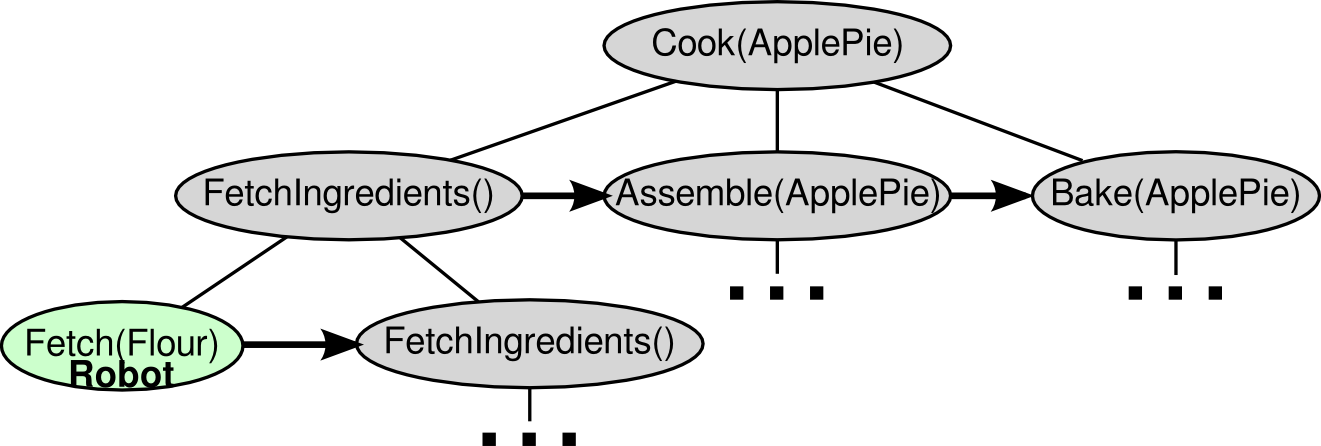
\includegraphics[width=0.77
 \textwidth]{img/plan.png}
%   \vspace{-10pt}
 \caption{Extrait d'un arbre de décomposition pour cuisiner une tarte aux pommes.}
 \label{fig:treePlan}
 \end{figure}
 
Pour prendre l'expertise en compte lors de la planification, une nouvelle règle sociale est nécessaire. L'objectif est de sélectionner le meilleur plan adapté à la politique choisie. Nous proposons deux politiques: la préférence de l'enseignement où l'être humain peut apprendre du robot, ou le choix de l'efficacité. Avec la politique de l'enseignement, le planificateur tente de produire des plans afin de maximiser le nombre de tâches humaines où l'humain a l'occasion d'apprendre, alors que l'efficacité pousse le planificateur à sélectionner des plans avec le moins de tâches inconnues pour l'être humain, afin de veiller à ce qu'il puisse être plus efficace (le robot peut cependant s'assigner certaines tâches inconnues à l'homme).
Dans le cas d'une politique visant à favoriser l'efficacité, la règle est tout simplement d'appliquer une pénalité à chaque fois qu'un humain doit effectuer une action qu'il ignore. Cette pénalité serait inversée pour la règle de l'enseignement.

Pour illustrer notre planification et la nouvelle règle sociale nous prenons l'exemple où un être humain et un robot doivent cuisiner une tarte aux pommes. Une partie du plan solution est représenté sur la figure \ref{fig: treePlan}. Dans ce contexte, on peut considérer que l'homme sait comment mener à bien toutes les actions (prendre, poser, couper, et ainsi de suite), mais il se peut qu'il ignore  l'ordre exact des différentes étapes de préparation (tâche de niveau supérieur). Si nous sommes favorables à l'enseignement, le plan devrait contenir un moyen de réaliser la recette avec un niveau de connaissance minimal sur chaque tâche et, autant que possible, l'homme sera en charge de ces étapes. D'autre part, si nous sommes favorables à l'efficacité, le plan devrait contenir la plus petite quantité de tâches inconnues à effectuer par l'utilisateur.
En utilisant cette règle, le robot est capable d'adapter sa génération du plan à la connaissance de l'utilisateur concernant les tâches contenues dans le plan partagé.
% Et les tâches peuvent être exécutées par l'un des agents. L'un à être effectivement choisi dépendra du reste du plan (optimalité de la répartition des tâches).
Pour calculer correctement le coût d'un plan, le planificateur considère également la connaissance d'une tâche comme améliorée après qu'elle ait été ajoutée au plan. Cela permet, lors de l'utilisation de la politique d'efficacité, de préférer les plans qui réutilisent de nombreuses fois la même tâche en l'affectant à un même utilisateur en réduisant le coût pour les prochaines occurrences. Par opposition, si différentes tâches sont utilisées ou si l'agent change en cours de route, le coût sera plus élevé. Ceci permet de prendre en compte la connaissance acquise au cours de l'exécution lors du calcul de coût.

Le planificateur est intégré dans un système de dialogue qui permet de négocier des plans (voir la section \ref{sec:planNego}). Plus précisément, il permet de poser des questions sur les préférences des utilisateurs et leurs capacités à accomplir une tâche. Si l'utilisateur indique au système qu'il ne peut pas effectuer une tâche donnée, elle ne sera pas ajoutée au plan ou tout du moins ne lui sera pas attribuée (invalidation de la condition préalable de la tâche correspondante).
En ce qui concerne les préférences des utilisateurs, l'étape de la négociation mettra à jour une base de données avec les préférences exprimées par l'utilisateur. Si l'utilisateur spécifie qu'il veut (ou non) effectuer certaines tâches, ces tâches, si elles sont ajoutées au plan et lui sont assignées, auront une récompense importante (respectivement pénalité) au niveau des coûts. Par conséquent, les plans qui contiennent de telles tâches seront considérés comme indésirables. Cependant, s'ils sont les seuls solutions possibles (en raison de l'incapacité, etc.), ils seront conservés et le planificateur donnera comme solution l'un de ces plans avec le moins de tâches indésirables et le maximum de tâches voulues attribuées à l'homme.

% To illustrate our planner and the new social rule let us consider the toy example where a human and a robot have to cook an apple pie. A part of the solution plan is shown in Figure \ref{fig:treePlan}. In this context we can consider that the human knows how to carry out all the actions (pick, place, cut, and so on) but they may not know the exact order of steps (higher level task). If we favor teaching, the plan should contain a way to achieve the recipe with a minimal knowledge level on each task and, as much as possible, human will be in charge of those steps. On the other hand, if we favor efficiency the plan should contain the smallest amount of unknown tasks to be performed by the user.
% Using this rule, the robot is able to adapt its plan generation to the knowledge of the user concerning tasks contained in the shared plan.
% %, and the tasks can be carried by either of the agents. The one to be actually chosen will depend on the rest of the plan (optimality of the task allocation).
% To properly compute the cost of a plan, the planner will also consider a task knowledge as upgraded once it is added to the plan. This allows the efficiency policy to prefer plans that reuse the same task many times and assign it to the same user to lower the cost, over some plans where different tasks are performed or the same task is performed by a different agent.

% The planner is integrated in a dialog system that allows to negotiate plans (see below). More precisely it allows for asking about user preferences and abilities. If the user tells the system that she/he cannot perform a given task, it will not be added to the plan (invalidate the corresponding task precondition).
% Concerning user preferences, the negotiation step will update a database with the preferences expressed by the user. If the user specifies that she/he (does not) want to perform certain tasks, those tasks if added to the plan, will take an important reward (resp. penalty) cost. Hence plans which contain such tasks will be considered as unwanted, however if they are the only possible solutions (because of inability and so on) they will be kept and the planner will return the one with the least number of unwanted and maximum number of wanted tasks.

%%%%%%%%%%%%%%%%%%%%%%%%%%%%%%%%%%%%%%%%%%%%%%%%%%%%%%%%%%%
% end HTN

\section{Présentation et négociation du plan partagé}
\label{planPresentation}

% intro
Une fois que le système robotique a généré un plan collaboratif adapté à la politique choisie (prenant en compte l'apprentissage, les capacités et les préférences), le plan doit être partagé avec le partenaire humain.
La parole est une "modalité puissante pour l'entretien continu de l'interaction coopérative" \cite{Lallee2013}. En effet, Tomasello suggère même que la principale fonctionnalité du langage est d'établir et de négocier des plans coopératifs \cite{tomasello2005}.
En considérant cela, nous décidons d'utiliser la parole pour présenter le plan au collaborateur.

\subsection{Prétraitement du plan}
L'arbre HTN généré représente une solution pour accomplir le but. Cependant, il se peut qu'en l'état il ne convienne pas à la présentation ou à l'explication du plan au collaborateur, car il peut contenir des étapes de raffinement qui rendraient l'explication confuse. Pour adapter le plan à l'explication nous utilisons deux règles.
%
(1) Nous retirons les tâches récursives. Si un nœud $n$ de l'arbre HTN contient la même méthode (en utilisant la fonction $compare$) que son parent $parent(n)$, il sera remplacer dans l'arbre par ses enfants $children(n)$. (2) Nous remplaçons également les nœuds avec un enfant unique par cet enfant.
\begin{enumerate}
\item $\textbf{if}$ $(compare(n, parent(n)))$ \textbf{then} $n \leftarrow children(n)$
\item $\textbf{if}$ $(children(n).size() = 1)$ \textbf{then} $n \leftarrow children(n)$
\end{enumerate}
Ces règles permettent de construire un arbre plus léger à traiter.
Ces traitements sont illustrés par la figure \ref{fig:pretraitement}.

\begin{figure}[ht!]
 \centering
 %  \vspace{-8pt}
  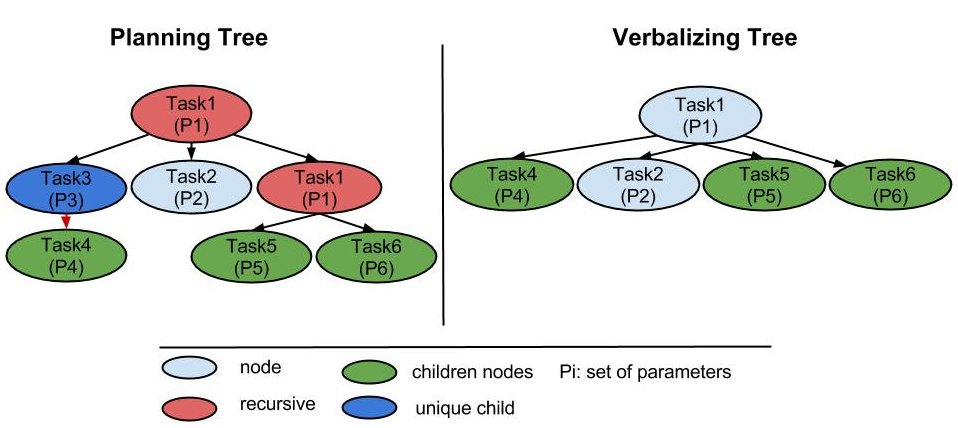
\includegraphics[width=0.99 \textwidth]{img/rules2.jpg}
%   \vspace{-10pt}
 \caption{Schéma expliquant le prétraitement de l'arbre de planification pour l'adapter à la verbalisation.}
 \label{fig:pretraitement}
 \end{figure}

\subsection{Présentation de plan}
%Miki: Could simplyfi in which agents are in charge of the task, removing the parhentesis.

Avant de pouvoir commencer l'exécution du plan, le robot présente le plan à l'homme et les allocations des tâches de haut niveau pour donner un aperçu global du plan. Une génération de langage naturel (NL pour Natural Language) est utilisée comme présenté dans le tableau \ref{table:pie-present}. 
Pour assurer le bon fonctionnement du système avec des plans de différentes tailles (scalability), lors de la présentation du plan, le robot verbalise seulement les  $N$ premières tâches de haut niveau. Par simplicité nous avons choisi $N$=$3$. Ce chiffre a été choisi de façon empirique, en effectuant quelques tests lors du développement. Nous pensons qu'établir ce nombre de façon optimal nécessiterais de mener des investigations plus poussées, dépendant du domaine ou de l'utilisateur et de son aisance à accomplir les tâches. Le robot présente les $N$ premières étapes du plan, puis les exécute avec son partenaire. Une fois que cette exécution est achevée, le processus de présenter/négocier/exécuter se répète jusqu'à ce que le plan soit achevé ou abandonné.
% Put in a double colomn table
%\begin{tabular}{ll}
%   agents(root) $+$ have\_to $+$ root  & "We have to cook an apple pie." \\
%   introduce\_presentation & "I will tell you the steps." \\
%   agents(root.child[0]) $+$ first $+$ root.child[0] & "You will first fetch the ingredients," \\
%   then $+$ agents(root.child[1]) $+$  root.child[1] & "Then I will assemble the apple pie," \\
%   finally $+$ agents(root.child[2]) $+$  root.child[2] & "Finally you will bake the apple pie in the oven." \\


%\end{tabular}
 
 
 \begin{table}
 %\vspace{-10pt}
\centering
\scriptsize
\renewcommand{\arraystretch}{1.3}
\begin{tabular}{|c|c|}
\hline
   agents(root) $+$ have\_to $+$ root  & "We have to cook an apple pie." \\
   \hline
   introduce\_presentation & "I will tell you the steps." \\
   \hline
   agents(child[0]) $+$ first $+$ child[0] & "You will first fetch the ingredients," \\
   \hline
   then $+$ agents(child[1]) $+$  child[1] & "Then I will assemble the apple pie," \\
   \hline
   finally $+$ agents(child[2]) $+$  child[2] & "Finally, you will bake \\
   & the apple pie in the oven." \\
   \hline
\end{tabular}
\caption{Présentation d'un plan pour cuisiner une tarte aux pommes. \textit{root} désigne la racine de l'arbre et \textit{child} est la liste de ses enfants.}
 \label{table:pie-present}    
\end{table}
 

\subsection{Négociation de plan}
\label{sec:planNego}
Une fois que le robot a présenté les tâches principales et la répartition, il lui faut s'assurer que l'homme accepte ce plan partagé. Le robot va simplement demander l'approbation de l'homme et, en cas de désaccord, lui demander ce qui ne lui convient pas.
Dans la version actuelle de notre système, deux types de requêtes provenant de l'homme sont prises en charge. Premièrement, l'homme peut exprimer ses préférences. Cela peut être la volonté de faire une tâche qui est assignée au robot ou le refus d'accomplir une tâche qui lui est assignée. La seconde possibilité est d'informé le robot que l'utilisateur ne peut réaliser une action. Dans les deux cas, ces informations seront ajoutées au modèle de l'utilisateur et enregistrées dans la base de données. Le robot va en suite essayer de trouver un nouveau plan qui évitera à l'humain d'effectuer une tâche qu'il ne souhaite pas ou dont il n'est pas capable de réaliser. Ce nouveau plan sera alors présenté et le robot demandera à nouveau l'approbation de l'homme. Dans notre système, les préférences des utilisateurs ont un coût plus élevé que la politique employée (apprentissage ou efficacité) car nous considérons que l'utilisateur devrait avoir la décision finale.

% The other possibility is to inform the robot that the user cannot perform an action. This will be added to the user's model and stored in the database. The robot will then try to find a new plan that prevents the human from performing a task the user is not willing or able to perform. This plan will then be presented and the robot will ask again for the user's approval. In our system, the user's preferences have a higher cost than the teaching policy as we consider that the user should have the final decision.

\section{Exécution de plan adaptative}
\label{planExecution}

\subsection{Algorithme de gestion de plan}
\label{sec:algo}
Une fois que le plan a été présenté et accepté par le collaborateur, l'exécution peut commencer. Nous donnons l'algorithme pour l'exécution adaptative de plan, puis nous donnons les explications associées.



%    \vspace{-12pt}
% \begin{program}
% \mbox{\textbf{$execute\_tree$ algorithm:}}
% %\seq{node parent, list<node> currentNodes};
% \FOR $n:=nodes.start$ \TO $n:=nodes.end$
%      $verbalize(n)$;
%      \IF $agents(n) = {robot}$
%         \THEN \IF $children(n)$ \neq \emptyset \AND $userKn(n) = NEW$
%         \AND $teachPolicy$
%           \THEN $execute\_tree(children(n))$;
%           $userKn(n) := BEGINNER$;
%         \ELSE $execute(n)$;  \FI
        
%      \ELSIF $userKn(n) = NEW$
%        \THEN $explain(n)$;
%          \IF $children(n)$ \neq \emptyset
%            \THEN $execute\_tree(children(n))$;
%                  $userKn(n) := BEGINNER$;
%          \ELSE $monitor(n)$; \FI
         
%      \ELSIF $userKn(n) = BEGINNER$
%        \THEN \IF $proposeExplain(n)$
%            \THEN $userKn(n) = NEW$;
%            (...);\rcomment{\textit{//Same process as NEW}}
%            \ELSE $monitor(n)$; \FI
%    %          userKn(n) = INTER; \FI
             
%        \ELSIF $userKn(n) = INTERMEDIATE$ 
%        \OR $userKn(n) = EXPERT$)
%          \THEN monitor(n); \FI
%  %        \IF(userKn(n) = INTER)
%  %          userKn(n) = EXPERT; 
% %\rcomment{This text will be set flush to the right margin}
% \end{program}
%    \vspace{-5pt}



\begin{algorithm}
\begin{algorithmic}[1]
\For{n$:=$nodes.start to n$:=$nodes.end}
	\If{$agents$(n) = \{robot\}}\label{alg:onlyRobotStart}
    	\If{$children(n) \neq \emptyset$ $\wedge$ $user\_kn(n)$ = NEW\par
        \hskip\algorithmicindent $\wedge$ $teachPolicy$}
        	\State $execute\_tree(children(n))$
            \State $user\_kn(n) :=$ BEGINNER
        \Else
         	\State $execute(n)$
        \EndIf\label{alg:onlyRobotEnd}
    \ElsIf{$user\_kn(n)$ = NEW}\label{alg:newStart}
     	\State $explain(n)$
        \If{$children(n)$ $\neq \emptyset$}
          	\State $execute\_tree(children(n))$
            \State $user\_kn(n)$ $:=$ BEGINNER
        \Else
         	\State $monitor(n)$
        \EndIf\label{alg:newEnd}
    \ElsIf{$user\_kn(n)$ = BEGINNER}\label{alg:beginnerStart}
      	\If{$propose\_explain(n)$}
          	\State $user\_kn(n)$ $:=$ NEW
            \State $(\dots)$ \Comment{Same process as NEW}
        \Else
          	\State $monitor(n)$
        \EndIf\label{alg:beginnerEnd}
    \ElsIf{$user\_kn(n)$ = INTERMEDIATE\par
    \hskip\algorithmicindent $\vee$ $user\_kn(n)$ = EXPERT}\label{alg:interStart}
      	\State $monitor(n)$
    \EndIf\label{alg:interEnd}
\EndFor
\end{algorithmic}
\caption{$execute\_tree(n)$}

\end{algorithm}



\begin{itemize}
\item \textit{$execute\_tree(n)$} est la fonction principale pour la gestion de l'exécution. Celle-ci est appelée après le processus de négociation. Elle a pour paramètre \textit{$nodes$}, une liste de nœuds initialement remplie avec les  enfants du nœud racine du HTN.
\item \textit{$teachPolicy$} est un booléen qui permet de définir si nous voulons utiliser la politique d'enseignement ou d'efficacité.
\item \textit{$agents(n)$} cette fonction renvoie la liste d'agents impliqués dans le nœud \textit{n} (plus précisément impliqués dans la tâche liée au nœud).
\item \textit{$verbalize(n)$} cette fonction permet de verbaliser la tâche courante, en utilisant le contexte du nœud pour la présenter (e.g. en utilisant des relations séquentielles tel que "first" (premièrement), "then" (puis) ou "finally" (enfin) en fonction de la position du nœud dans la liste).
\item \textit{$user\_kn(n)$} cette fonction donne le niveau de connaissance de l'utilisateur concernant la tâche \textit{n}.
\item \textit{$propose\_explain(n)$} cette fonction va conduire le robot à proposer une explication pour la tâche courante. Si l'utilisateur accepte l'explication, la fonction renvoie "true" et "false" sinon.
\item \textit{$explain(n)$} cette fonction lance une procédure pour expliquer la tâche actuelle à l'utilisateur. Cette procédure peut être implémentée comme un script pour lancer une vidéo, une explication verbale, ou même de demander à un expert d'expliquer la tâche.
\item \textit{$monitor(n)$} cette fonction envoie une requête au système de supervision pour qu'il suive l'exécution du nœuds courant afin de s'assurer qu'elle se déroule correctement. Si la requête renvoie un succès, cela signifie que la tâche correspondant au nœud a été effectuée correctement. Par conséquent la fonction améliorera la connaissance de l'humain puis la fonction \textit{$execute\_tree$} continue de s'exécuter. Dans le cas d'un échec, la fonction dégradera le niveau de connaissance de l'utilisateur, la fonction \textit{$execute\_tree$} sera stoppée, et va renvoyé une erreur qui va entraîner une requête de replanification au superviseur et une nouvelle exécution si un plan est trouvé.
\item \textit{$execute(n)$} cette fonction procède de façon similaire à la fonction de suivi (monitor(n)). La différence est qu'elle envoie une requête pour que le robot exécute le nœud.
\end{itemize}
 
\subsection{Explication de l'algorithme de gestion de plan}
Pendant l'exécution, nous utilisons l'arbre HTN pré-traité pour réaliser le plan, donner des explications et surveiller la réalisation des tâches en fonction du niveau de connaissance de la tâche contenue dans la modèle de l'humain.
Nous utilisons une procédure d'exploration du plan en profondeur, ou "depth first search" pour procéder durant l'exécution. Cela permet de donner le contexte à la tâche à accomplir.
Lorsque le processus atteins un nœud, plusieurs situations peuvent se présenter.
% Monitor function is responsible for: knowledge update(success = upgrade, fail = downgrade) and replan in case of failure. 

\subsubsection{Le robot est le seul impliqué (lignes ~\ref{alg:onlyRobotStart}-~\ref{alg:onlyRobotEnd})} si le robot est le seul agent en charge du nœud courant, si le collaborateur a un niveau de connaissance égal à \textit{NEW} pour la tâche actuelle et si la politique choisie pour l'interaction est l'apprentissage, le robot va exécuter les sous tâches en mode "démonstration", ce qui signifie qu'il va verbaliser chaque tâche-enfant avant de la réaliser. Une fois la tâche accomplie, le robot mets à jour la connaissance de l'homme sur le nœud courant en lui donnant la valeur \textit{BEGINNER}. La même procédure sera appliquée aux enfants, afin que le robot verbalise chaque tâche qui doit être apprise par le collaborateur (et uniquement celles-ci).
Si le robot est en charge du nœud, mais que le collaborateur humain a déjà les connaissances suffisantes sur le nœud, ou que la politique d'interaction est l'efficacité, le robot ne verbalisera que la tâche de plus haut niveau qu'il a à accomplir.

Dans le cas où l'humain est impliqué dans le nœud courant, le comportement du robot va dépendre des connaissances de l'humain sur la tâche, car il se peut que le robot doive expliquer celle-ci ou adapter la surveillance des tâches à accomplir par l'homme.
L'explication pourrait se faire de différentes manières: en montrant une vidéo, en demandant à un expert d'expliquer la tâche ou simplement en guidant verbalement l'utilisateur, étape par étape. Nous donnerons des détails sur l'explication verbale du robot à l'utilisateur car c'est la méthode qui implique réellement le robot.

% if new
\subsubsection{Le collaborateur est \textit{NEW} (lignes~\ref{alg:newStart}-~\ref{alg:newEnd})} si l'humain a un niveau \textit{NEW} pour la tâche actuelle, le robot l'explique.
Lorsque le robot guide verbalement l'utilisateur, si le nœud courant a des enfants, nous allons plus profondément dans l'arbre et appliquons à nouveau le comportement approprié en fonction du niveau de connaissance aux nœuds enfants. Si le nœud actuel n'a pas d'enfant (est une feuille), le superviseur attends que l'utilisateur accomplisse l'action courante. En cas de succès, le niveau de connaissance pour la tâche est mise au niveau \textit{BEGINNER} (dans l'algorithme ci-dessus, cette étape est faite dans la fonction \textit{monitor}).


%When verbally guiding the user, if the current node has only one child node, we  go deeper in the tree and apply again the corresponding behavior according to the knowledge level. If the current node is actually an operator (a leaf), the supervisor waits for the user to perform the current action. In case of success, the knowledge level for the task is upgraded to \textit{BEGINNER} (in the above algorithm this is done in the \textit{monitor} process).

% if beginner
\subsubsection{Le collaborateur est \textit{BEGINNER} (lignes ~\ref{alg:beginnerStart}-~\ref{alg:beginnerEnd})} si l'humain a un niveau de connaissance à \textit{BEGINNER} pour la tâche courante, nous demandons s'il a besoin d'explications. Si c'est le cas, nous dégradons son niveau de connaissance, pour la tâche actuelle, à \textit{NEW} et appliquons le même procédé que le niveau \textit{NEW}. Si l'utilisateur refuse les explications, le robot va simplement surveiller l'exécution du nœud courant, sans aller plus profondément dans l'arbre. En cas de succès, le niveau de connaissance pour la tâche courante est amélioré pour être mis à \textit{INTERMEDIATE}. Ce niveau de connaissance (\textit{BEGINNER}) sera également utilisé comme niveau par défaut. De cette façon, lorsque le niveau de connaissance de l'utilisateur est inconnu sur la tâche, nous demanderons tout simplement s'il a besoin d'explication et le robot adaptera son comportement en fonction de sa réponse.

% if intermediate
\subsubsection{Le collaborateur est \textit{INTERMEDIATE} (lignes~\ref{alg:interStart}-~\ref{alg:interEnd})} si l'humain a un niveau  \textit{INTERMEDIATE} pour la tâche courante, le robot verbalise la tâche courante et ne propose pas de l'expliquer, car l'homme a réussit à faire au moins une fois la tâche sans explications. D'autre part, nous n'allons pas plus loin dans l'arbre et surveillons directement la tâche courante. Si l'utilisateur échoue, le robot dégrade son niveau de connaissance à \textit{BEGINNER}, sinon il l'améliore en \textit{EXPERT}.

% if expert
\subsubsection{Le collaborateur est \textit{EXPERT} (lignes~\ref{alg:interStart}-~\ref{alg:interEnd})} dans le cas du niveau \textit{EXPERT}, sur la tâche courante, nous procédons comme le niveau de connaissance précédent, en dégradant à \textit{INTERMEDIATE} si l'utilisateur fait une erreur et en gardant le niveau \textit{EXPERT} s'il l'accomplit comme prévu.

\subsection{Exécution et surveillance}
Une fois que la tâche actuelle à effectuer a été expliquée, le robot l'effectue si elle lui est allouée, ou il surveille l'accomplissement de la tâche par son partenaire humain. Par conséquent, la surveillance peut être faite à un haut niveau d'abstraction si l'humain a suffisamment de connaissance.
Nous avons choisi cette adaptabilité au niveau de la surveillance car nous pensons que le robot sera plus efficace, préservant ses ressources en concentrant son attention plus souvent sur les parties du plan qui n'ont jamais été exécutées par le partenaire humain, et moins souvent lorsqu'il a une certaine forme d'expertise, donnant également plus de liberté à l'homme sur la façon d'effectuer la tâche qu'il connaît (par exemple en changeant l'ordre des sous-tâches).

Surveiller les actions humaines est un problème complexe, particulièrement avec des tâches de haut-niveau, où nous ne suivons pas une suite d'actions atomiques. Le système devrait avoir des modèles de raisonnement pour permettre au robot de comprendre si l'état du monde est cohérent avec l'action que l'humain doit accomplir. Il devrait également être capable de mesurer le niveau d'engagement de l'humain à la tâche, afin de mieux estimer si l'humain est en train d'accomplir ou non sa partie du plan partagé, et réagir de manière appropriée.



\subsection{Échec et replanification}

Le but de suivre les actions humaines est d'être capable de gérer les comportements imprévus de l'homme et rétablir l'interaction. Lorsque cela arrive, le robot doit informé l'homme de son comportement considéré comme faux et dégrader son niveau de connaissance. La prochaine fois que l'humain réalisera cette tâche, le robot va le guider et surveiller son exécution à un niveau plus détaillé (les tâches enfants).
Le planificateur de tâche reçoit une requête pour calculer un nouveau plan pour atteindre le but avec le nouvel état du monde. 
Un des bénéfices de cette mise à jour dynamique des connaissances de l'homme est que ce nouveau plan peut comprendre des tâches que le robot a déjà expliqué ou que l'humain a effectué avant que l'échec ne se produise. Dans ce cas, guider l'humain à travers l'exécution du nouveau plan sera plus rapide car le robot n'aura pas à ré-expliquer ces tâches.
Ce comportement de replanification permet de donner de la robustesse au système robotique et permet une procédure de recouvrement socialement acceptable où nous informons l'humain de l'erreur et ré-expliquons le plan seulement avec le niveau de détails nécessaires.
%, as we took into account his knowledge improvement during the execution that failed.




%%%%%%%%%%%%%%%%%%%%%%%%%%%%%%%%%%%%%%%%%%%%%%%%%%%%%%%%%%%%%%%%%%%%
% end supervisor

%%%%%%%%%%%%%% START IMPLEMENTATION
% Maybe discuss here about the scenario and all and then in user study say that we use the same scenario.
\section{Implémentation}
\subsection{Architecture}
Nous avons implémenter les mécanismes proposés dans notre architecture\footnote{Open-Source modules: http://homepages.laas.fr/gmilliez/hri2016/}. La figure \ref{fig:architecture} illustre l'architecture et les interactions entre les modules principaux.
Le module de gestion de l'exécution du HTN (\textit{htn execution manager}) contient l'algorithme présenté en section \ref{sec:algo}.
Il est contrôlé par le superviseur et envoie des requête au superviseur pour surveiller ou exécuter une tâche.

Pour nos tests, nous utilisons le PR2 de Willow Garage\footnote{https://www.willowgarage.com/pages/pr2/overview}. Comme la perception n'est pas l'aspect principal de ces travaux, nous utilisons simplement la Motion Capture pour suivre les humains, et un système de reconnaissance de tag pour le suivit d'objets.
Au commencement du scénario, le robot scan l'environnement, ce qui lui permet de construire un modèle de l'état du monde.
% TODO Make it fit better
Nous avons choisi pour cette première implémentation une stratégie simple de surveillance. Le robot observe l'environnement, mets à jour son modèle d'état du monde en conséquence, et surveille les conséquences attendues des actions. Les actions réalisées sont inférées en utilisant la distance entre le bras de l'homme et un point d'intérêt (par exemple une boîte). Nous considérons une action comme "échouée" si elle n'a pas été réalisée avant une durée prédéfinie.

%
%
%
\begin{figure}[ht!]

 \centering
 \begin{tabular}{cc}
  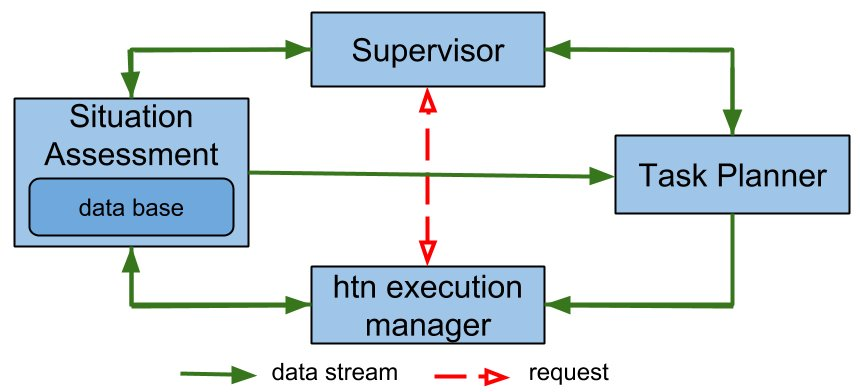
\includegraphics[width=0.69\textwidth]{img/archi.jpg}
 \end{tabular}
  % \vspace{-10pt}
 \caption{Architecture du système permettant d'adapter la collaboration aux connaissances du partenaire humain.}
 \label{fig:architecture}
 %  \vspace{-20pt}
 \end{figure}
 
 \subsection{Expérimentation}
 \label{sec:experiment}
Pour tester notre système, nous avons choisi un scénario où un humain revient du travail et doit préparer deux desserts qu'il compte apporter à un dîner. Il décide de cuisiner une tourte aux pommes et une tarte à la banane, mais il n'a pas de connaissances préalable sur la façon de les cuisiner. Il demande à son robot domestique des indications et son aide comme illustré par la figure \ref{fig:scenarioPie}.

\begin{figure}[ht!]

  %\vspace{-6pt}
 \centering
 \begin{tabular}{cc}
  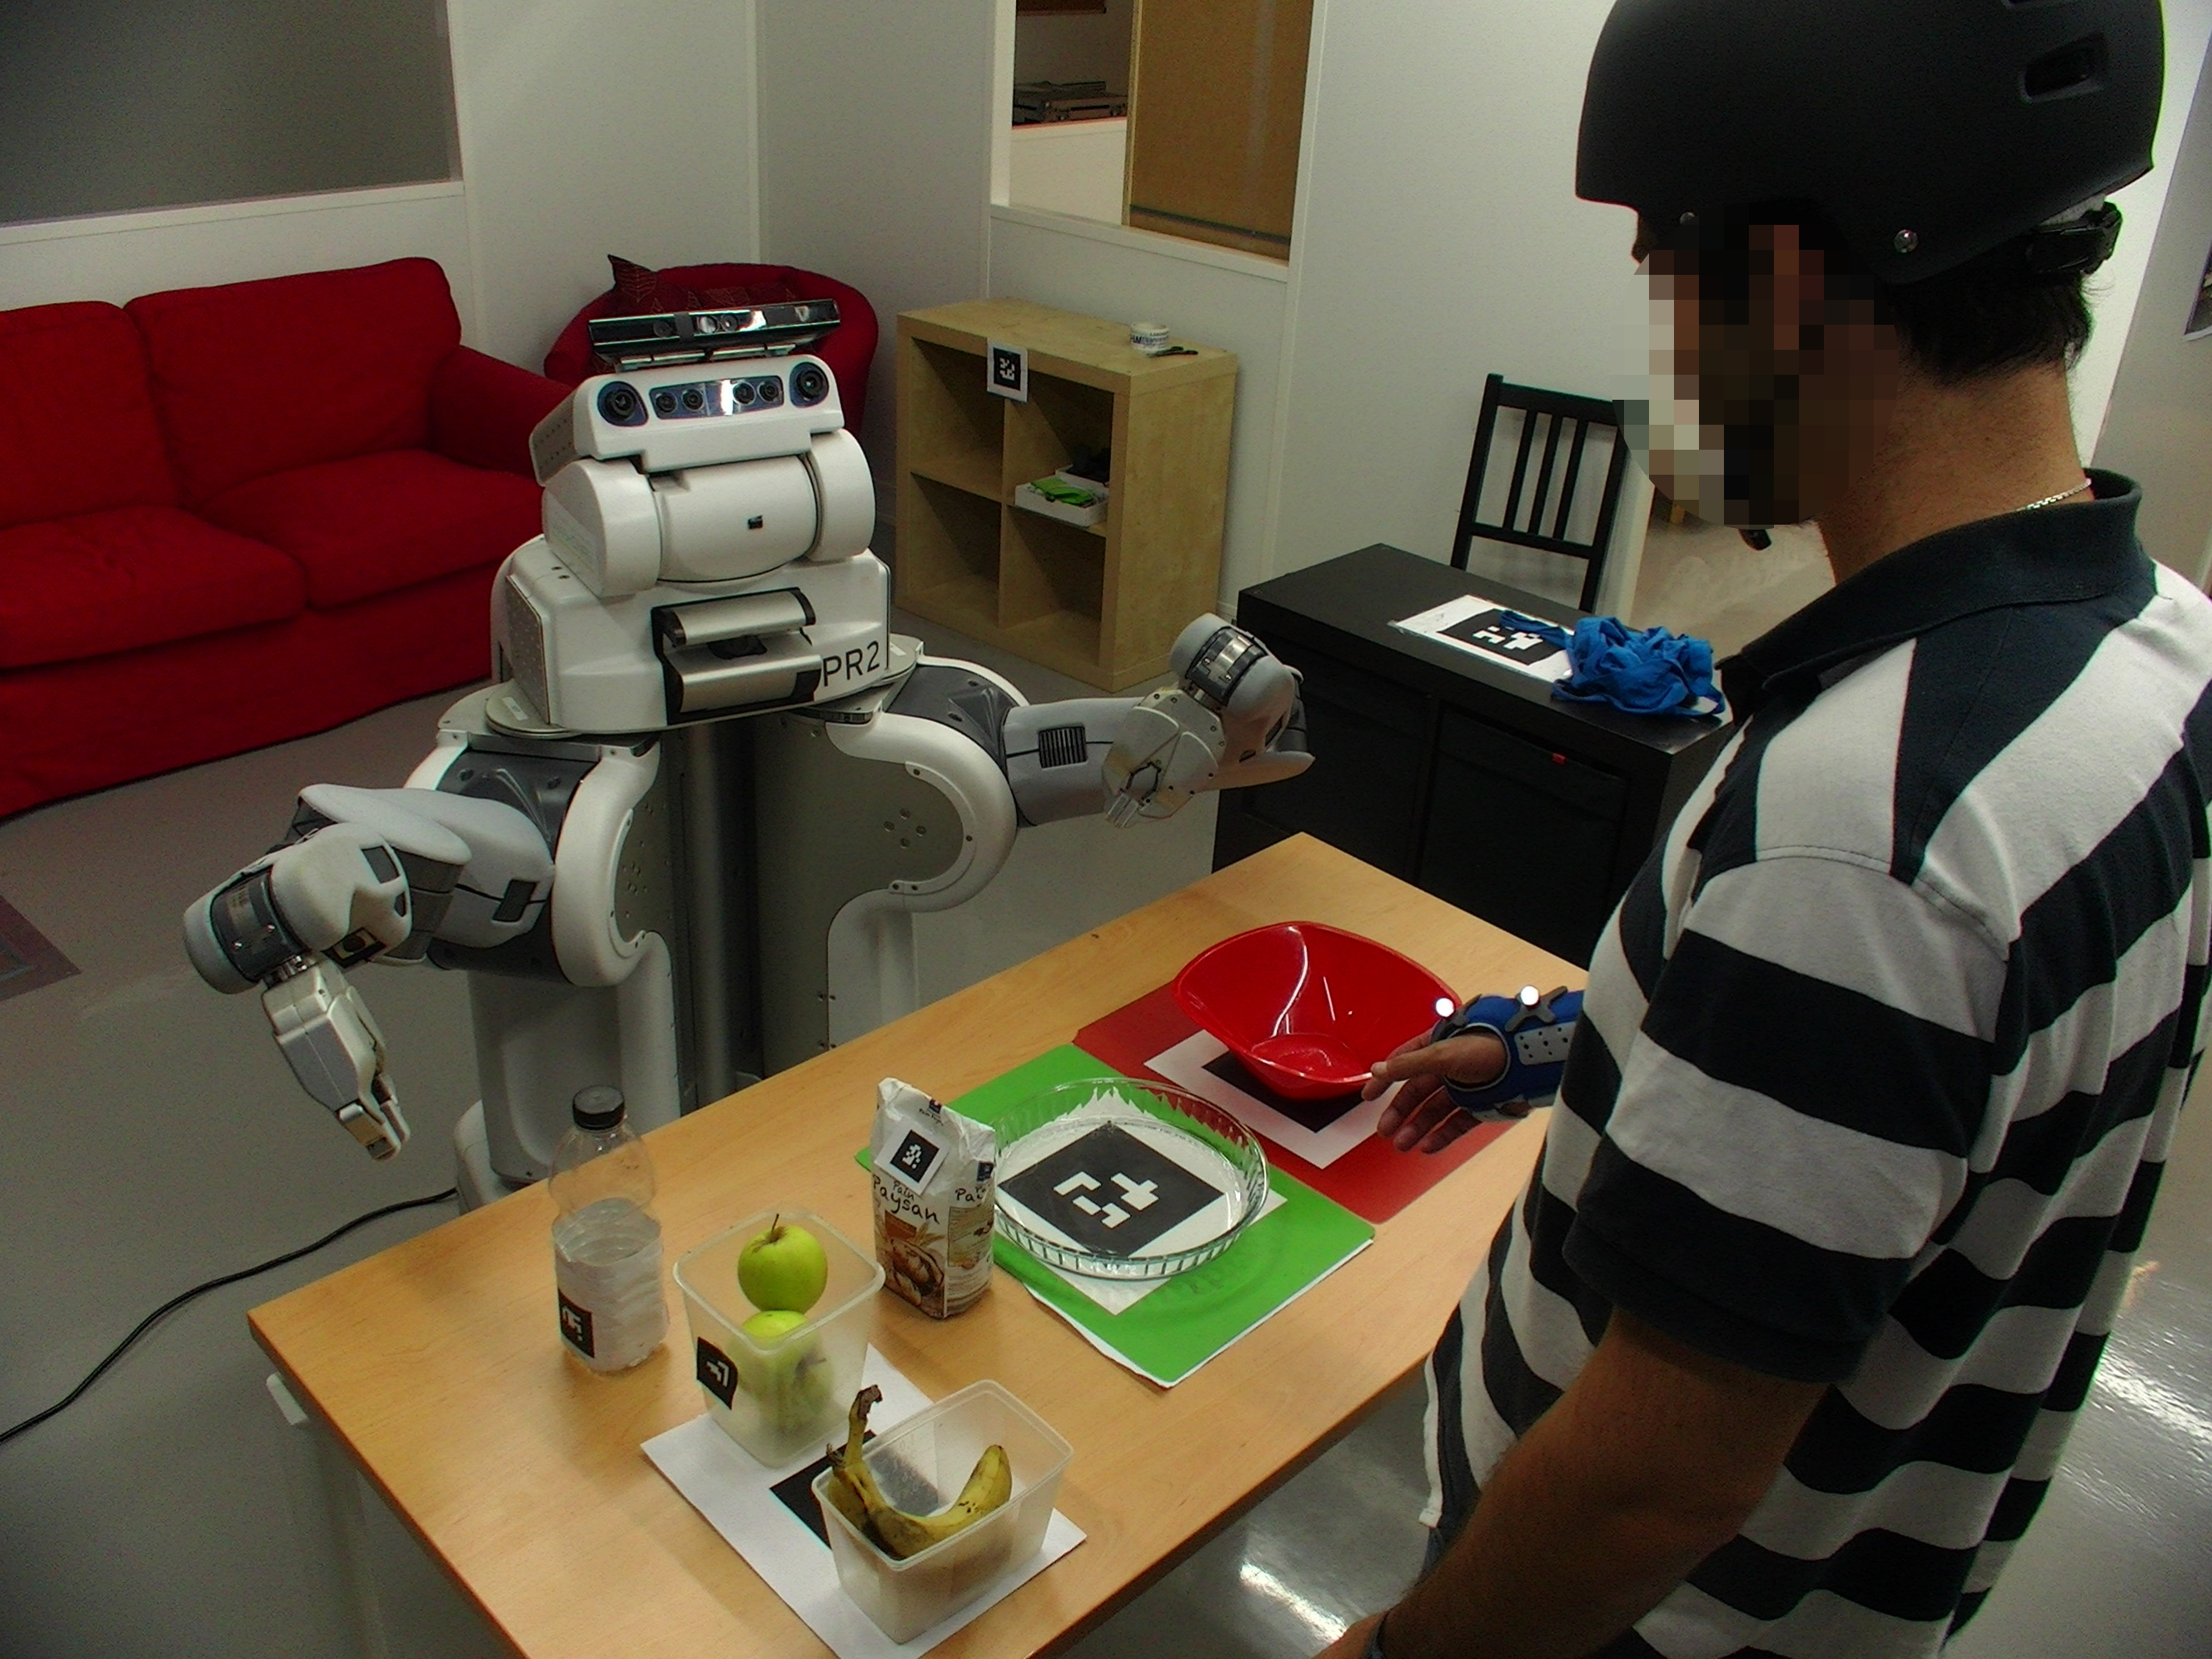
\includegraphics[width=0.69\textwidth]{img/scenario.JPG}
 \end{tabular}
  % \vspace{-6pt}
 \caption{Illustration du scénario de préparation de la tarte aux pommes.}
 \label{fig:scenarioPie}
  % \vspace{-10pt}
 \end{figure}

Comme dans ce scénario l'utilisateur est pressé, nous allons utiliser la politique d'efficacité.
Nous avons créer un domaine représentant la connaissance nécessaire sur les tâches à utiliser par le planificateur de tâches (\textit{task planner}) et pour le gestionnaire d'exécution d'htn (\textit{htn execution manager}).
Pour cuisiner la tourte aux pommes, cinq tâches principales sont nécessaires. Nous imaginons dans ce scénario, qu'à cause de limitation au niveau de l'accessibilité, le robot ne peut faire la pâte ou préparer les fruits. De ce fait, la répartition de tâche sera la suivante.




\begin{itemize}
\item L'humain va préparer la pâte, ce qui signifie qu'il va la faire et la mettre dans le moule.
\item Le robot va préparer la mixture, ce qui signifie qu'il va la faire et la mettre dans le moule.
\item L'humain va alors préparer les fruits, en les coupant et en les mettant dans le moule.
\item Puis il va prendre en charge la pâte pour le haut de la tourte.
\item Enfin, le robot s'occupera de la cuisson en mettant la tourte dans le four et en réglant la minuterie.
\end{itemize} 

Après la première étape, l'humain aura acquis la connaissance pour faire la pâte. Par conséquent, pendant l'exécution, lors de l'étape de la seconde pâte (pour le haut de la tourte), le robot demande à l'utilisateur s'il a besoin d'aide. Nous supposons ici qu'il dit "non". Le robot n'explique donc pas cette étape et l'humain atteindra le niveau \textit{INTERMEDIATE} après l'avoir accomplie. Concernant la deuxième tâche humaine, elle sera représentée dans le modèle de connaissance comme \textit{$<$human1, PrepareFruits, [fruit], VALUE$>$}. En effet nous considérons que le processus est le même pour n'importe quel fruit (les couper, puis les mettre dans le moule) donc nous utilisons la classe fruit plutôt que l'instance pomme ou banane.
%
%MB give the task representation to explain class / instance
%

Après avoir cuisiner le premier dessert, à savoir la tourte aux pommes, le robot génère un plan pour cuisiner la tarte à la banane. Cette fois-ci, nous considérons que les deux agents peuvent accomplir toutes les tâches (tout est atteignable pour les deux parties). La tarte à la banane requière les même tâches avec différents paramètres. La mixture est différente, ainsi que les fruits mais la méthode de préparation de ceux-ci est la même (coupé et répartir dans le moule). De plus, la tarte à la banane n'aura pas de pâte sur le dessus et aura un temps de cuisson différent. Le plan généré est présenté dans la figure \ref{fig:bananaPlan}. Nous pouvons observer que la politique favorise l'efficacité en donnant les tâches connues à l'utilisateur (\textit{PrepareDough} et \textit{PrepareFruits}). Pendant l'exécution, comme l'utilisateur a un niveau de connaissance à \textit{INTERMEDIATE} sur comment préparer la pâte, le robot ne va pas l'expliquer. Concernant la tâche de préparation de fruits (\textit{prepareFruits}), le robot va proposer de fournir des explications à l'humain car celui-ci ne l'a accomplie qu'une fois avec des explications.


%TODO: try to add streams?
\clearpage

\begin{sidewaysfigure}[t!]
%   \vspace{-10pt}
 \centering
 \begin{tabular}{c}
  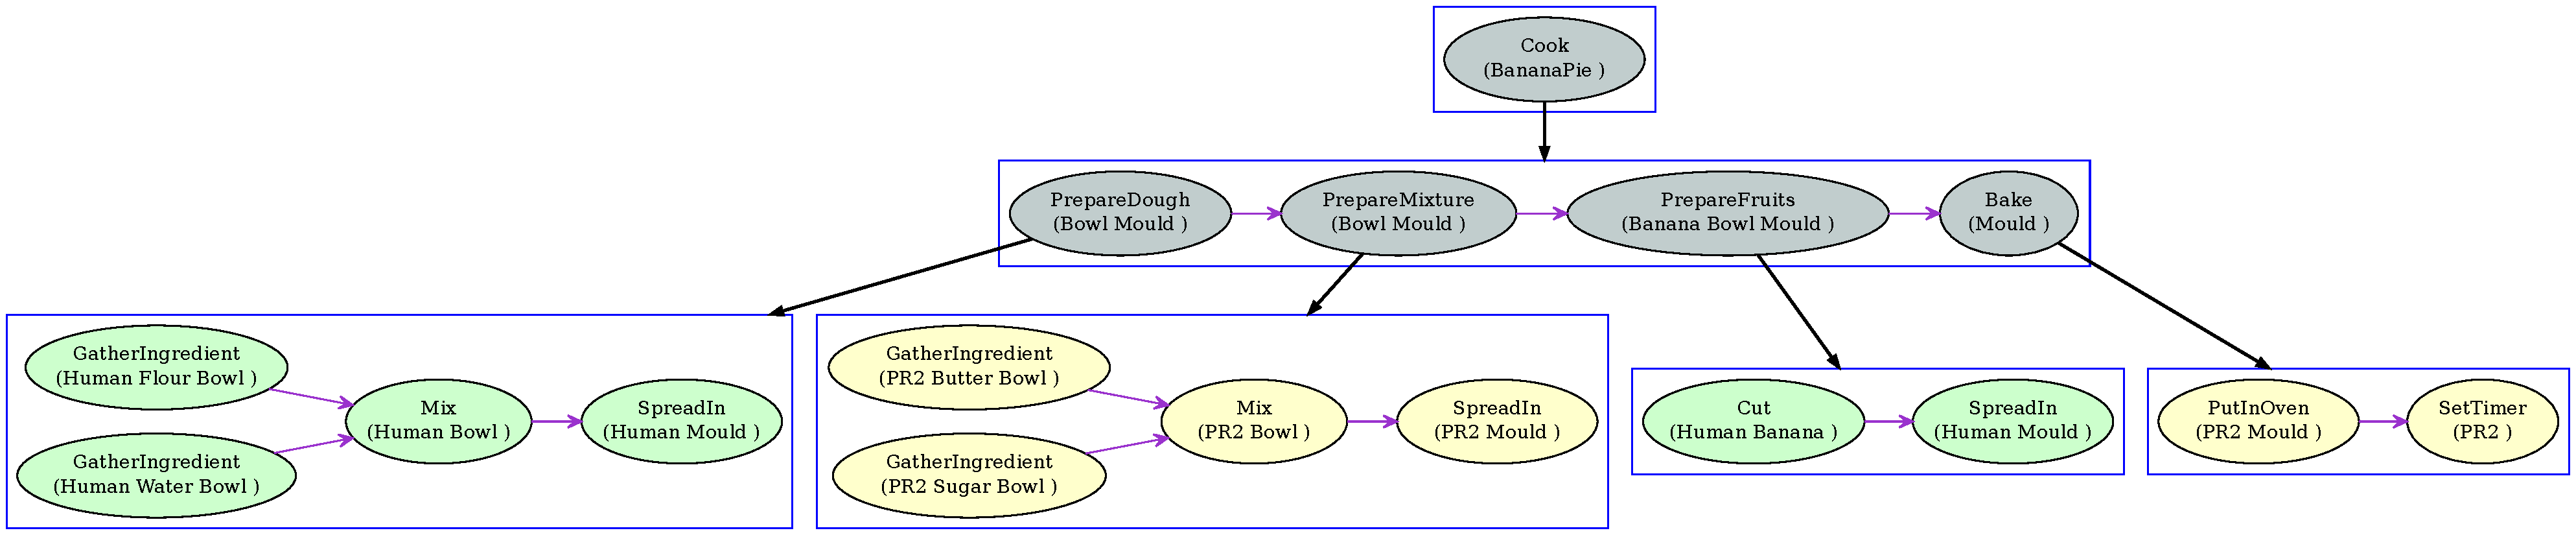
\includegraphics[width=1.0\textwidth]{img/bananaPie.pdf}
 \end{tabular}
 \caption{L'arbre HTN associé au plan partagé généré pour réaliser la tarte à la banane de façon collaborative.}
 \label{fig:bananaPlan}
 %  \vspace{-10pt}
\end{sidewaysfigure}


\clearpage


% \begin{figure*}[ht!]

% %   \vspace{-20pt}
%  \centering
%  \begin{tabular}{cc}
%   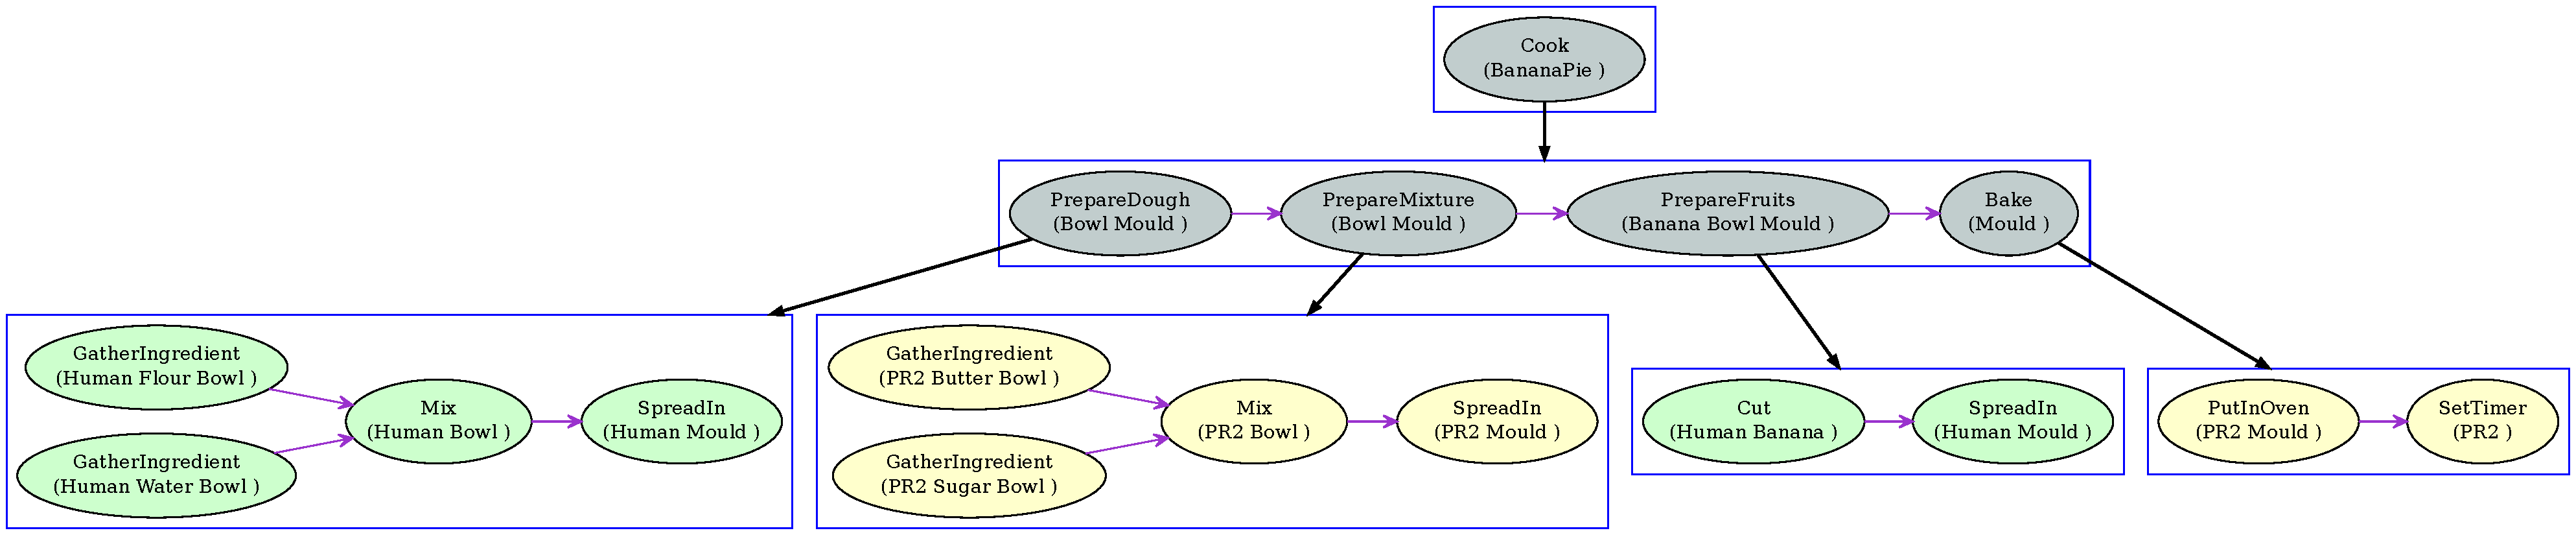
\includegraphics[width=0.99\textwidth]{img/bananaPie.pdf}
%  \end{tabular}
%   % \vspace{-8pt}
%  \caption{Plan partagé et l'HTN associé généré pour réaliser la tarte à la banane de façon collaborative.}
%  \label{fig:bananaPlan}
%   % \vspace{-22pt}
%  \end{figure*}
 


%TODO: mb show some dialogue here, or describe the process? Plan generation, explanation, replan. Mb say that robot task were simulated?

%%%%%%%%%% END IMPLEMENTATION

\section{Étude utilisateur et discussion}
\label{study}

\subsection{Étude utilisateur}
Nous avons conduit une étude comparative afin d'avoir une première évaluation de la façon dont l'adaptabilité du système est perçue par les utilisateurs. Deux groupes d'utilisateurs ont été constitués, auxquels il a été demandé de suivre le scénario des deux desserts. Le premier groupe a interagit avec un robot simulé équipé d'un système basique (BS). BS a le même comportement que notre système, à ceci prêt qu'il n'a pas le mécanisme permettant de connaître le niveau de connaissance de l'homme. Le deuxième groupe interagit avec un second système, appelé système de connaissance (KS pour Knowledge System), exhibant un comportement similaire à celui fournit par notre système.
Tous les participants ont par la suite évalué l'interaction sur plusieurs critères.
%
La répartition de tâche présentée dans la section \ref{sec:experiment} 
est utilisée dans les deux systèmes pour accomplir l'exemple de la tourte aux pommes. Une fois qu'ils ont cuisiné le premier dessert, le robot génère un plan pour cuisiner la tarte aux pommes. Dans KS, le robot a le même comportement que notre système et favorise une répartition de tâches pour la tarte à la banane où l'humain doit accomplir les tâches qu'il a déjà accomplies lors de la préparation de la tourte aux pommes (préparant la pâte et les fruits).
Dans BS, nous imaginons que le robot pourrait demander à l'humain de faire la mixture plutôt que la pâte.

Deux groupes composés chacun de 19 participants, de 18 à 60 ans, ont été constitués. Chaque groupe a interagit avec un des systèmes. Cela a été réalisé grâce à une étude utilisateur en ligne\footnote{Étude utilisateur KS http://goo.gl/forms/qvbtu4vcFW, et BS http://goo.gl/forms/ZSvGcCi5le}, où nous avons présenté des images de l'état de la tâche et des enregistrements des paroles du robot en Français pour chaque étapes de l'interaction (comme présenté dans la figure \ref{fig:user_study}).
Pour certaines étapes, l'utilisateur pouvait choisir l'action à réaliser, rendant possible d'effectuer une action fausse conduisant à une replanification du robot. Par soucis de simplicité, la replanification était limité à une annulation de l'action erronée avant de reprendre le plan précédent. De plus, pour se concentrer sur l'adaptabilité de notre solution grâce à la prise en compte des connaissances de l'homme dans les différentes étapes du plan partagé, nous n'avons pas autoriser la négociation avec l'utilisateur et le robot a directement imposé son plan.
À la fin de l'interaction simulée, nous avons posé les mêmes questions aux deux groupes, concernant l'adaptabilité du système et le partenaire robotique.
Les utilisateurs ont donné des notes en suivant une échelle de Likert de un (pas d'accord) à 5 (d'accord) afin d'exprimer leur ressentit sur plusieurs affirmations (comme indiqué dans la figure \ref{fig:user_study}).
Par exemple, une des questions était "Avez-vous eu l'impression que le robot adaptait ses explications au niveau de connaissance que vous avez acquis au cours de l'interaction?".

\begin{figure}[ht!]
  %\vspace{-8pt}
 \centering
 \begin{tabular}{cc}
  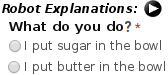
\includegraphics[width=0.48\textwidth]{img/ustudy9.png} &
  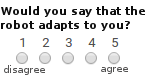
\includegraphics[width=0.38\textwidth]{img/ustudy11.png}
 \end{tabular}
 % \vspace{-6pt}
 \caption{L'utilisateur écoute un enregistrement de la voix du robot et choisit l'action à faire (image de \textit{Gauche}). À la fin, l'utilisateur évalue l'interaction en utilisant une échelle de Likert (\textit{image de droite}.}
 \label{fig:user_study}
 %  \vspace{-15pt}
 \end{figure}

\subsection{Résultats}

Nous avons recueilli les résultats pour chaque groupe d'utilisateurs, et calculer la moyenne ainsi que l'écart type et la p-valeur pour évaluer la fiabilité. La p-valeur a été calculée en utilisant une t-distribution avec 18 degrés de liberté et en considérant que la moyenne des notes pour KS serait plus haute que pour BS comme énoncé de notre hypothèse et que la moyenne des notes pour les deux groupes serait identique comme hypothèse nulle.
%We compare below the results for each system. 
La figure \ref{fig:results} résume les résultats obtenus en affichant la moyenne des notes, l'écart type sous forme de barres d'erreurs ainsi que la p-valeur. En comparant les réponses des utilisateurs, nous pouvons voir que l'adaptation du robot au niveau de connaissance de l'homme concernant les explications fournies est bien perçue avec une moyenne de 3.74 pour KS contre 2.05 pour BS. Les utilisateurs interagissant avec KS ont globalement remarqué que la répartition des tâches prenait en compte leur connaissance en donnant une notation moyenne de 3.42 pour KS et 2.58 pour BS. La dernière question concerne la liberté de choisir la manière d'accomplir une tâche, liée au suivi de plus haut niveau en cas de connaissance suffisante de la tâche. La moyenne est de 2.58 pour KS contre 1.89 pour BS, et la p-valeur est inférieur à 0.05. On peut donc conclure que même sur cet aspect l'adaptabilité a été perçue.
%As some users just performed the task as the robot teach them, they may not have noticed that they could perform it in a different way. However, 
Avec le système KS, les utilisateurs ont attribué une moyenne de 3.11 pour l'adaptabilité globale du système contre 1.89 pour le système basique.
Nous avons également demandé comment le partenaire robotique était perçu. Bien que en BS le robot ne soit pas perçu comme plus verbeux (2.53 pour KS contre 2.47 pour BS), il semble que les utilisateurs ont trouvé l'interaction légèrement plus naturelle (2.74 contre 2.42) et le robot est apparu comme plus intelligent (2.79 contre 2.26). Même si ces résultats renforcent notre idée, comme la p-valeur est supérieur à 0.1 pour l'aspect naturel, cela ne permet pas de prouver qu'il y a une différence notable entre les deux système (cela ne permet pas de rejeter l'hypothèse nulle).
Nous pensons que d'autres paramètres ont été pris en compte par les utilisateurs, comme la parole elle-même, ce qui a conduit les utilisateurs des deux expériences à évaluer l'interaction comme étant peu naturelle. Améliorer la verbalisation avec l'usage d'un dictionnaire de synonymes pourrait aider à avoir des résultats plus significatifs.


 \begin{figure}[ht!]

 %  \vspace{-9pt}
 \centering
 \begin{tabular}{cc}
  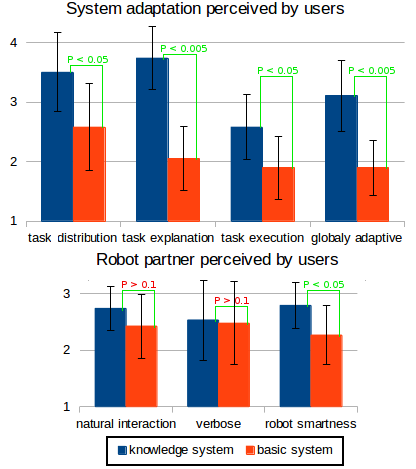
\includegraphics[width=0.81\textwidth]{img/respvalue3.png}
 \end{tabular}
 %  \vspace{-8pt}
 \caption{Notes moyennes des utilisateurs sur plusieurs critères concernant la perception de l'adaptation du système par rapport à leur connaissance  (en haut) et concernant le partenaire robotique (en bas). Les résultats en bleu représente l'évaluation de notre système (KS) et en rouge un système basique (BS.}
 \label{fig:results}
 % \vspace{-10pt}
 \end{figure}

Cette étude permet de montrer comment les utilisateurs ont pu percevoir l'adaptation du robot à leur niveau de connaissance concernant la répartition de tâches, les explications fournies, et la surveillance de leur actions. De plus, le robot est apparut comme plus intelligent. Cependant ces premiers résultats doivent être confirmés par une étude sur une population plus grande. De même, comme travaux futurs nous envisageons de conduire une étude utilisateur avec un vrai robot car nous pensons que cela permettra d'avoir des avis plus réalistes de la part des utilisateurs.
Dans les deux études, nous avons demander aux participants comment l'interaction pourrait être améliorée selon eux.
Plusieurs utilisateurs ont suggéré qu'ils aimeraient choisir quelles actions faire ou non, mettant en valeur l'importance de la négociation (nous avions retiré la négociation de l'étude utilisateur pour nous concentrer sur l'adaptation au niveau des connaissances). L'un des utilisateurs a suggéré qu'il aimerait pouvoir être informé de l'évolution du plan de temps en temps. 
Cela peut facilement être ajouté car à chaque moment le robot connaît le nombre de nœuds qu'il reste dans le plan partagé pour accomplir le but.
D'autres utilisateurs ont fait des suggestions concernant la parole du robot, la voix, l'intonation et le choix des mots. Ces aspects ne sont pas l'objet de l'étude, cependant ces commentaires montrent leur importance pour l'interaction avec l'homme.

%
% It would be good to have at least some metrics (number of words/ length of interaction/ explanation with/ without knowledge)
% Some feedback from users?

%%%%%%%%%%%%%%%%%%%%%%%%%%%%%%%%%%%%%%%%%%%%%%%%%%%%%%%%%%%%%%%%%%%%%

%Is this needed? Or in conclusion?
%\section{perspective on future work}




\section{Conclusion}
Dans ce chapitre nous avons présenté une solution pour permettre à un robot de gérer une activité de collaboration homme-robot, et ce de la génération de plan à l'exécution, en guidant son partenaire humain de manière efficace et socialement acceptable.
Notre approche est basée sur un suivi dynamique et une mise à jour en ligne des connaissances du partenaire humain. 
Nous avons également mis en place deux politiques d'interaction, l'apprentissage ou l'efficacité, qui procurent différents niveaux d'interactions. 
Notre méthode incorpore le suivi des actions humaines de haut niveau, en se focalisant sur la complétion de la tâche plutôt que sur la façon dont la tâche est accomplie. Cela permet de donner une certaine flexibilité à l'humain lorsqu'il réalise les tâches qui lui sont assignées.

%In the future we would like to conduct a user study enlightening the necessity of segmentation of the plan verbalization and execution according to the number of actions to verbalize for each partner to ensure scalability of our solution.
Nous avons mener une étude comparative en ligne. Les résultats sont encourageants, les utilisateurs ont été capables de percevoir l'adaptabilité du robot sur les aspects de génération, d'accompagnement et de surveillance de tâches.
%
À l'heure actuelle, cette approche nécessite que le robot connaisse toutes les méthodes à réaliser (incluant la décomposition de chaque tâche). Ajouté la possibilité d'enseigner une décomposition de tâches au robot comme dans  \cite{Mohseni2015} permettrait de surmonter cette restriction.
Pour la partie de négociation, nous avons fournit un premier mécanisme, en donnant un coût différent à une tâche lorsque l'utilisateur exprime son souhait de la faire ou non. Cependant, cela pourrait être amélioré en utilisant des travaux précédents tel que \cite{chu2000conflict} qui expose une infrastructure de Proposition/Évaluation/Modification pour prendre en charge la négociation.
Il serait par exemple intéressant de prendre en compte, une fois de plus, la connaissance de l'utilisateur pour accepter ou refuser une proposition de modification. Le robot pourrait ainsi informé l'utilisateur de la différence de coût pour effectuer une tâche entre l'homme et le robot (une tâche pourrait être plus ou moins simple ou dangereuse selon qu'elle est effectuée par un agent humain ou robotique).
En ce qui concerne la surveillance de tâches humaines, l'implémentation actuelle utilise une stratégie simple basée sur l'estimation du résultat d'une tâche après un certain temps. Nous souhaiterions améliorer cela en concevant des mécanismes plus élaborés pour estimer l'engagement de l'homme dans une tâche et mieux reconnaître lorsqu'une tâche surveillée a échoué. L'humain pourrait aussi informer le robot pourquoi il n'est pas en train d'effectué la tâche attendue.
Enfin, pour améliorer l'interactivité, il serait pertinent d'autoriser l'humain à demander directement des explications sur les actions du robot comme dans  \cite{Lomas2012}.
%Explaining robot actions \cite{Lomas2012}
%https://www.researchgate.net/publication/254007903_Explaining_robot_actions

%human explaining his choice
%Telling more than we can know: Verbal reports on mental processes
%http://people.virginia.edu/~tdw/nisbett&wilson.pdf


\ifdefined\included
\else
\bibliographystyle{acm}
\bibliography{These}
\end{document}
\fi